\graphicspath{{sections/03_CAPO_Optimization/}}

\chapter{CAPO: Control and Actuator Placement Optimization for Large-Scale Problems with Nonlinear Dynamics}
%
% \titlerunning{CAPO: Control and Actuator Placement Optimization}
% % If the paper title is too long for the running head, you can set
% % an abbreviated paper title here
% %
% \author{Mitchell B. Fogelson\inst{1} %\orcidID{0009-0000-0938-4491}
% \and
% Giusy Falcone\inst{2}
% %\orcidID{0000-0001-6194-5559}
% \and
% Zachary Manchester\inst{1}
% %\orcidID{0000-0002-3071-7091}
% }
% %
% \authorrunning{M.B. Fogelson et al.}
% % First names are abbreviated in the running head.
% % If there are more than two authors, 'et al.' is used.
% %
% \institute{Carnegie Mellon University, Pittsburgh, PA, USA \\  \and
% University of Michigan, Ann Arbor, MI, USA \\ Corresponding Author Email: \email{mfogelson@cmu.edu}}
% %
% \maketitle              % typeset the header of the contribution
%
Actuator selection and placement are critical aspects of robot design that are tightly coupled to task performance. Jointly optimizing actuator placement and control policies or trajectories can enhance efficiency and robustness. However, current optimization methods struggle to scale to high-dimensional systems with many degrees of freedom, including soft robots, large flexible spacecraft, or cloth manipulation.
We propose CAPO, a scalable Control and Actuator Placement Optimization method that jointly optimizes the number, type, and placement of actuators, along with control trajectories. CAPO concurrently optimizes over all the control and design parameters in a single computationally tractable nonlinear program that scales favorably with system size and complexity.
CAPO is evaluated against a state-of-the-art genetic algorithm and mixed-integer programming solvers on six problems, including an acrobatic multirotor aircraft, a spinning space structure, cloth manipulation, and a soft robotic swimmer. On small-scale problems, CAPO finds comparable solutions with similar objective values in 2.5-218x less time than existing methods. On large-scale problems, CAPO is the only method capable of finding a feasible solution, and it achieves actuator configurations that reduce the total number of actuators by 12\%-27.5\% compared to baselines.

% \keywords{Control Theory and Optimization  \and Optimal Control \and Design Optimization}
%
%
%
\section{INTRODUCTION}

Nature provides many examples of physical structures adapted to perform a behavior efficiently. For instance, humans can swim long distances, but are much slower than dolphins. Similarly, the design of a robotic system significantly influences its ability to complete tasks, as demonstrated by Boston Dynamics’ Atlas robot being one of the few humanoids to perform a backflip \cite{noauthor_leaps_nodate}. From a designer’s perspective, creating a backflipping robot requires significant effort and many iterations to select and place actuators. From the control engineer’s perspective, significant effort is applied to enable the robot to achieve the backflip while operating within the constraints of the selected actuators. Within the robotics community, the type and placement of actuators are essential factors in robot design across various applications and tasks, from soft robot locomotion \cite{Bhatia2021} to maneuvering continuum robots \cite{baykal_asymptotically_2019, a_kuntz_kinematic_2018, c_bergeles_concentric_2015, t_anor_algorithms_2011, j_-t_lin_generalized_2022, morimoto_toward_2018, s_niyaz_optimizing_2019} and resource-constrained robot control \cite{Seifried2012}. 

Actuator selections from a set of options are discrete choices that expand the design space combinatorially as the number of actuators considered grows. Design and control optimization are typically performed in separate sequential loops, resulting in inefficient evaluation of intermediate designs. Direct collocation (DIRCOL) is an optimal control method used to determine open-loop control trajectories that minimize a cost function while adhering to dynamics and actuator constraints. DIRCOL optimizes state and control variables simultaneously, making it well-suited for handling complex nonlinear dynamics \cite{hargraves1987}. A unique feature of DIRCOL is that intermediate iterations in the optimization loop do not need to be dynamically feasible; only the final result is required to satisfy all constraints. Including parameters like actuator type and position as decision variables in DIRCOL can mitigate the costly evaluation of intermediate designs.

A simplified diagram showing the joint actuator and control optimization problem can be seen in Figure \ref{fig:simple_example}. Applying these parameters in a DIRCOL formulation and solving the joint problem of actuator selection and control optimization problem leads to a mixed integer nonlinear program (MINLP), which is NP-hard \cite{olshevsky2014minimal}. This makes it computationally impractical to find globally optimal solutions in most cases. Thus, designing efficient algorithms that can quickly find feasible sub-optimal solutions while scaling to large problems is a crucial area of research in robotics. 

% In many cases, the downstream tasks and behaviors for the robot are predetermined, and addressing the problem of control and design holistically has been demonstrated to improve reference tracking, lower design costs, and simplify control complexity \cite{Spielberg2017}.

  % parameters do not always have relaxations to continuous variants, but it can increase design optimization efficiency by not having to evaluate all intermediate designs.  

% The joint problem of actutor selection and control optimization leads to Mixed Integer Nonlinear Program (MINLP). 

 % and  

% The core challenge of task-driven robot design is simultaneously designing a controller and determining which actuators to place in which locations to minimize a user-specified cost function.  \todo{let's ease into this a little by talking about how actuator selection is discrete/integer while control design and placement are continuous, so you get a MINLP.} 

% Similar selection-and-placement challenges arise in many different applications, such as wireless sensor networks \cite{tossa2022area}, structural health monitoring \cite{tan2020computational}, high-speed UAV sensors \cite{yang2019optimization}, and actuators for large flexible space structures \cite{Maghami1993}. 
%There are many large-scale robotics problems with high degrees of freedom that would greatly benefit from a tool like this, such as the design and control of a large flexible spacecraft, manipulating a deformable cloth, and soft robotic locomotion.
 % A unique challenge of task-driven robot design on top of the actuator placement is solving for a closed-loop control policy that can satisfy the desired goal. The actuator placement and control policy are coupled and should be solved for simultaneously. It has been proven that minimal controllability problems are NP-hard \cite{olshevsky2014minimal}, so determining the optimal amount of actuators that can find a valid control policy is unattainable for design problems. Since the general problem is computationally intractable, designing efficient algorithms that can quickly find feasible sub-optimal solutions while scaling to large problems is a crucial area of research in robotics.

\begin{figure}
    % \vspace{-10pt}

    \centering
    % \includegraphics[width=0.6\linewidth]{figures/Rebuttal_figure_1_motivation.png}
    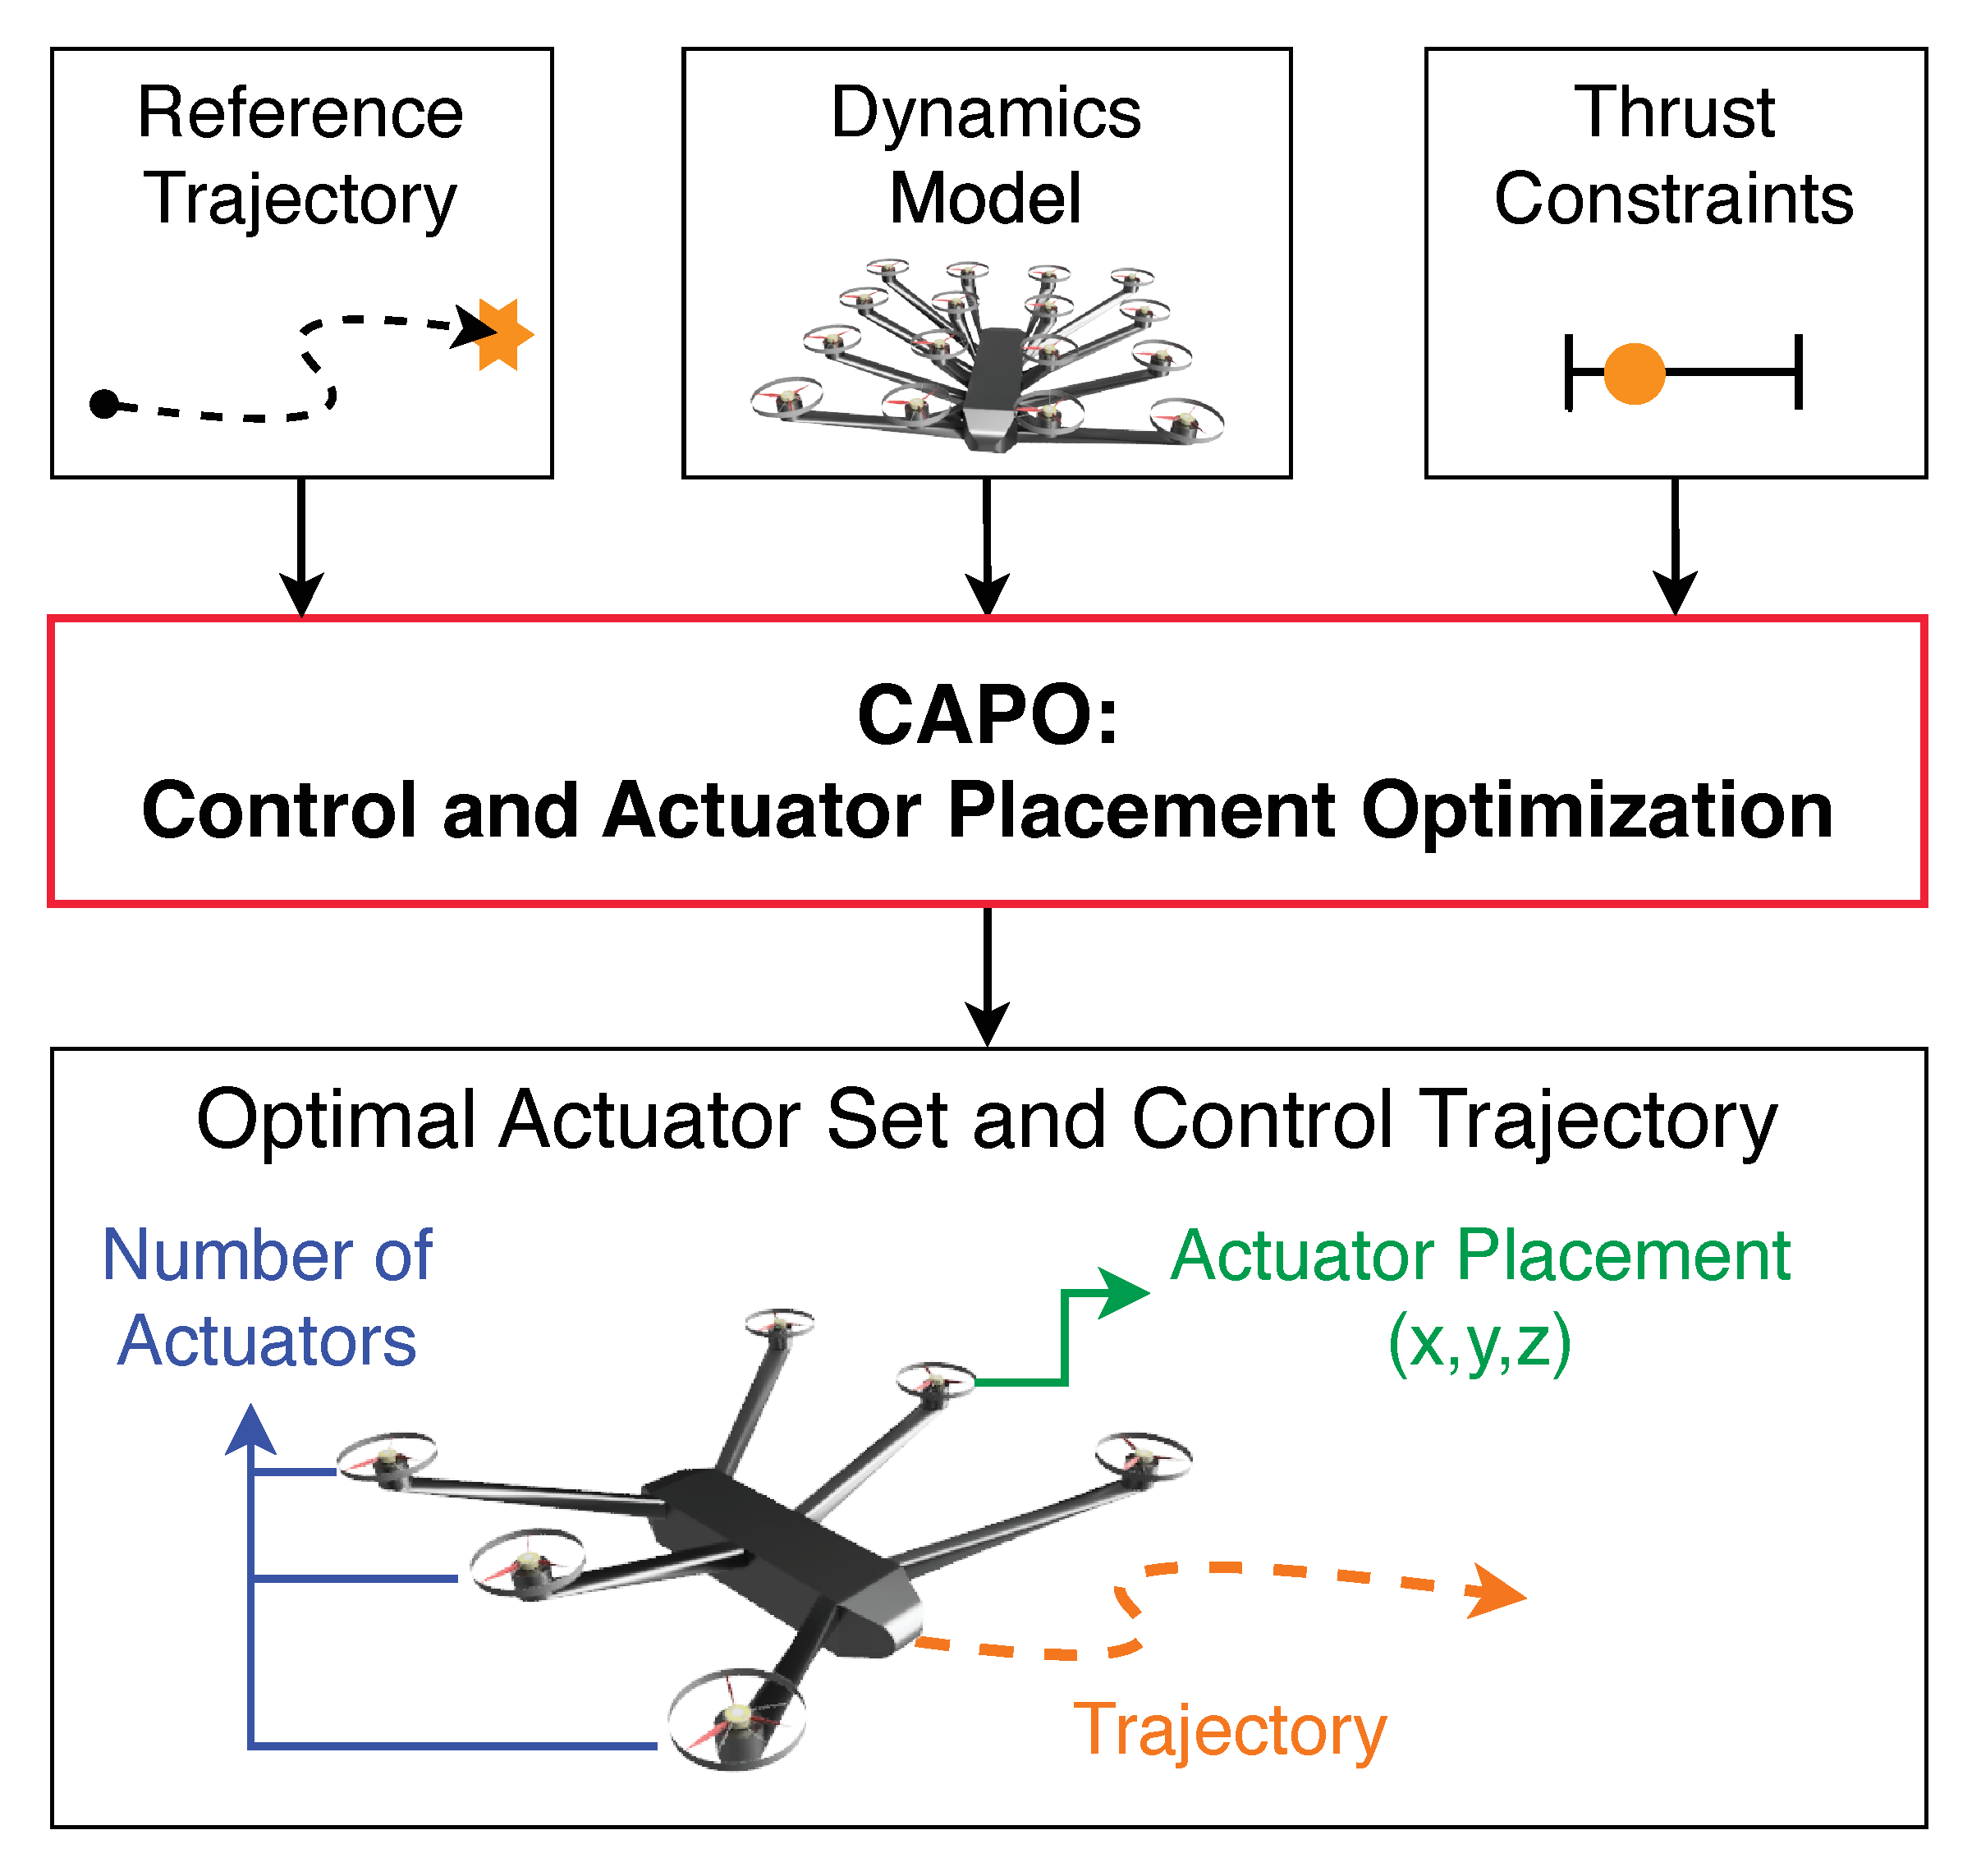
\includegraphics[width=0.6\linewidth]{figures/Figure_1_CAPO_motivation.eps}
    \caption{Example of joint robot-control-and-design optimization, which takes a user-defined reference trajectory, dynamics models, and thrust constraints as input, and outputs a feasible design configuration and control trajectory. %The diagram shows finding the optimal set and placement of propellers on a multirotor to achieve a flip and the open-loop control trajectory.
    }
    % \caption{A block diagram of actuator-type-and-location placement on a three-body space structure using idealized thruster and reaction-wheel actuators for space applications, placed at the centers of mass of the rigid bodies. The problems require the user to input a goal, model, and constraints, and output a constraint-satisfying system configuration.}
    \label{fig:simple_example}
    % \vspace{-15pt}

\end{figure}

To tackle the challenges of joint actuator and control optimization for robot design, we propose CAPO, a single-level optimization formulation for actuator placement and control that jointly minimizes the number of actuators, control effort, and tracking error to perform a desired task. CAPO achieves this by relaxing the actuator-placement problem into a computationally tractable nonlinear program (NLP), providing a framework that scales well for complex, high-dimensional robots and trajectories. To evaluate its performance, CAPO is compared to three state-of-the-art algorithms: a genetic algorithm (GA)\cite{wildart2022}, a mixed-integer quadratic program (MIQP) solver\cite{gurobi}, and a mixed-integer nonlinear program (MINLP) solver\cite{juniper}. These methods are compared in Table~\ref{tab:}, which highlights CAPO's advantages. We evaluate the methods on four low-dimensional actuator-placement design problems in simulation, including an over-actuated double integrator, an acrobatic multirotor aircraft, a flexible space structure, and a cloth-manipulation task. CAPO is further demonstrated on three additional high-dimensional problems that the other methods failed to solve, including a 120-degree-of-freedom (DoF) flexible space structure, a 150-DoF cloth-manipulation task, and a 234-DoF soft-robotic swimmer.
Our contributions include: %\todo{Claim the advantages over other methods here}
\begin{enumerate}
\item A scalable algorithm, CAPO, for the simultaneous control and actuator-selection-and-placement problem that concurrently considers actuator type, placement, and control parameters.
%\item {Introduction of additional decision variables to support time/trajectory invariant constraints.}
\item {A domain-randomization approach for improved design robustness that maintains problem sparsity structure and scalability.}
% \item \todo{This one isn't very clear without already knowing what's going on.} A continuous relaxation of the discrete actuator-type-and-placement problem with a feasible projection to enable solving larger scale problems than previously possible.
\item Experimental validation of CAPO on various high-dimensional robotics problems demonstrating its computational advantages over other state-of-the-art methods.
% \item Concurrent optimization of multiple sample trajectories to approximate an optimal control policy
%\item Formulation of the full dynamics with maximal coordinates to simplify the modeling of complex robots and trajectories while maintaining computational efficiency
\end{enumerate}
The paper proceeds as follows: Section \ref{sec:capo:background} reviews background information on nonlinear programming, integer-programming relaxations, and L1 regularization. Section \ref{sec:capo:related_works} surveys related works that address the actuator-placement problem. Section \ref{sec:capo:actuator_problem} formalizes the control-and-actuator-placement problem. Section \ref{sec:capo:capo_alg} derives the CAPO algorithm. Section \ref{sec:capo:experiment} provides implementation details and presents the experimental results. Finally, Section \ref{sec:capo:conclusions} summarizes the findings and proposes directions for future work.

% Please add the following required packages to your document preamble:
% \usepackage[table,xcdraw]{xcolor}
% Beamer presentation requires \usepackage{colortbl} instead of \usepackage[table,xcdraw]{xcolor}
% Please add the following required packages to your document preamble:
% \usepackage[table,xcdraw]{xcolor}
% Beamer presentation requires \usepackage{colortbl} instead of \usepackage[table,xcdraw]{xcolor}
\begin{table}[]
    % \vspace{-10pt}
\centering
\caption{Comparison table of the proposed method, CAPO, with three state-of-the-art approaches: Genetic Algorithm, Mixed Integer Quadratic Program, and Mixed Integer Nonlinear Program. CAPO's primary advantages are its ability to jointly optimize all parameters in a single problem, handle nonlinear constraints, and scale effectively to large numbers of binary variables.}
\resizebox{\textwidth}{!}{
\begin{tabular}{|c|c|c|c|c|}
\hline
& \textbf{\begin{tabular}[c]{@{}c@{}}\\ CAPO \\ (Ours)\end{tabular}} & \begin{tabular}[c]{@{}c@{}}Genetic\\ Algorithm\\ (GA)\end{tabular} & \begin{tabular}[c]{@{}c@{}}Mixed Integer\\ Quadratic Program\\ (MIQP)\end{tabular} & \begin{tabular}[c]{@{}c@{}}Mixed Integer\\ Nonlinear Program\\ (MINLP)\end{tabular} \\ \hline
Single Level                                                      & $\checkmark$                                      & $\times$                                         & $\checkmark$                                                        & $\checkmark $                                                         \\ \hline
\begin{tabular}[c]{@{}c@{}}Nonlinear \\ Constraints\end{tabular} & \checkmark                                      & $\checkmark$                                        & $\times{\color[HTML]{CB0000} }$                                  & $\checkmark $                                                         \\ \hline
\begin{tabular}[c]{@{}c@{}}Scalable to \\ High Dim.\end{tabular}  & \checkmark                                      & $\times $                                        & $\times$                                                         & $\times $                                                          \\ \hline
\end{tabular}
}
\label{tab:}
% \vspace{-20pt}
\end{table}

% \begin{figure*}
%     \centering
%     \includegraphics[width=\linewidth]{figures/Rebuttal_figure_2_benchmarks.drawio.png}
%     % \includesvg[width=\linewidth]{figures/Rebuttal_figure_2.drawio.svg}
%     \caption{CAPO is a single-level method for concurrent optimization of states, actuators, and controls with nonlinear constraints, contrasting with GA's bi-level structure that separates configuration generation and trajectory optimization. Both MIQP and MINLP are single-level approaches, but MIQP employs linearized and binary constraints, while MINLP uses nonlinear and binary constraints.}
%     % \caption{Comparison of CAPO to bi-level Genetic Algorithm (GA), Mixed-Integer Quadratic Programming (MIQP), and Mixed Integer Nonlinear Programming (MINLP) approaches. CAPO is a single-level concurrent optimization of states, actuators, and controls with nonlinear constraints. GA is a bi-level method with a lower-level configuration generator and upper-level trajectory optimization. MIQP is a single-level formulation with linearized constraints as well as binary constraints. MINLP is a single-level formulation with nonlinear constraints and binary constraints}
%     \label{fig:comparison_block diagrams}
%     % \vspace{-16pt}

% \end{figure*}
% \vspace{-5pt}
\section{Background} \label{sec:capo:background}
We now review background information on Linear and Nonlinear Programming, Mixed-Integer Programming, the branch and bound method for solving Mixed-Integer Programs, and the L1 regularization method for optimization. 
\subsection{{Linear, Nonlinear, and Mixed-Integer Programming}}
Smooth nonlinear programs (NLPs) can be expressed in the following standard form,
\begin{mini!}
{\textbf{x, y}}{\ell(\textbf{x, y})}
{\label{eq:optimization}}{}
\addConstraint{f(\textbf{x, y})}{= \textbf{0}}
\addConstraint{g(\textbf{x, y})}{\geq \textbf{0} ,}
\end{mini!}
where, $\textbf{x} \in \mathbb{R}^n$ and $\textbf{y} \in \mathbb{R}^m$ are decision variables, $\ell(\cdot)$ is a scalar-valued objective function, and $f(\cdot)$ and $g(\cdot)$ are equality and inequality constraints, respectively. Functions are assumed to be at least twice continuously differentiable.
If $\ell(\cdot)$, $f(\cdot)$, and $g(\cdot)$ are linear functions, the problem is known as a linear program (LP). If $\ell(\cdot)$ is quadratic and both $f(\cdot)$ and $g(\cdot)$ are linear, the problem is called a quadratic program (QP). In all of these cases, locally optimal solutions satisfy the Karush-Kuhn-Tucker (KKT) conditions (first-order necessary conditions) \cite{kuhn1950kkt}. %\todo{Check that this is correct}

A mixed-integer nonlinear program (MINLP) adds the constraint,
\begin{equation}
     \textbf{y}\in\{0, 1\}^m
     \label{eq:mip-binary}
\end{equation}
% \begin{mini!}
    % {\textbf{x, y}}{\ell(\textbf{x, y})}
    % {\label{eq:MIP}}{}
    % \addConstraint{f(\textbf{x, y})}{= \textbf{0}}
    % \addConstraint{g(\textbf{x, y})}{\geq \textbf{0}}
    % \addConstraint{x}{\in\mathbb{R}^n}
%     \addConstraint{\textbf{y}}{\in\{0, 1\}^m , \label{eq:mip-binary}}
% \end{mini!}
where the \textbf{y} variables are constrained to take on integer values. Note that, without loss of generality, we consider binary constraints $\textbf{y} \in \{0, 1\}^m$. Similar to the continuous case, if $\ell(\cdot)$, $f(\cdot)$ and $g(\cdot)$, are all linear functions, the problem is known as a mixed-integer linear program (MILP), with mixed-integer quadratic programs (MIQP) defined similarly. Mixed-integer programs are NP-hard in general, and their computational complexity grows combinatorially in the problem size \cite{yuan2016binary}.

The branch-and-bound method is a prevalent technique for solving mixed-integer programs \cite{land_automatic_1960}. In its basic form, branch and bound first relaxes the binary constraints \eqref{eq:mip-binary}, known as a continuous relaxation, then solves the relaxed problem to optimality.
% for the  \eqref{eq:mip-binary} become inequalities:
% \begin{equation}
%     \label{eq:C4_MIP_relax}
%     0\leq y \leq 1
% \end{equation}
This relaxed problem is strictly easier than the original binary-constrained version, and will have an objective value that lower bounds the original problem. The solution to this subproblem returns $(\textbf{x}^{(j)}, \textbf{y}^{(j)})$, where $j$ is the subproblem index. If all values of $\textbf{y}^{(j)}$ happen to take on values of 0 or 1, then the solution is also an optimal solution to the original MIP. If this is not the case, the problem is branched into two new problems for each element $y^{(j)}_i \notin \{0, 1\}$; one with the additional constraint $y_i=0$ and the other with the additional constraint $y_i=1$. The new subproblems are solved, and the branching continues until all values in the solution satisfy the original problem constraints. If a feasible solution is found, its objective value is used to prune branches that have relaxed solutions with higher objective values, as these branches cannot yield a better solution than the one already found. 

% As the number of binary variables increases, the potential branching factor increases exponentially. and many subproblems may need to be evaluated to find a constraint-satisfying solution.
% \vspace{-15pt}
\subsection{L1 Regularization Methods}
% \todo{Reviewer: "The reviewer encourages a brief survey of the use of LASSO in such design problems for clarifying the novelty of this formulation. "}
%Regularization is used in various applications to encourage sparse solutions (i.e. containing many zeros) to optimization problems. Two common regularization techniques are the L1 regularization, also known as the LASSO regression, and the L2 regularization, also known as Ridge regression.
One-norm or L1 regularization (also called ``LASSO regularization'') is commonly used in statistics and machine learning to drive many model coefficients to zero, producing sparse solutions \cite{efron2004lar, santosa1986linear, tibshirani1996regression, zou2005regularization, Candes2014}. L1 regularization presents itself as an additional penalty term in the objective function:
\begin{mini!}
    {\textbf{x}, \textbf{y}}{\ell(\textbf{x}, \textbf{y})+\sum_{i=1}^{m}\alpha|y_i|}
    {\label{eq:Lasso}}{}
\end{mini!}
where $\alpha$ is a scalar penalty weight. While this method is well-known and widely used in the statistics and machine-learning communities, it is less frequently applied in the design community. Notably, Ha et al. \cite{ha2018computational} and Skouras et al. \cite{Skouras2013} have utilized L1-regularization to promote sparsity in design-optimization applications. The hyperparameter $\alpha$ controls the sparsity of the solution, with larger values encouraging solutions with more zero elements. One may need to evaluate multiple $\alpha$ values to find a desirable solution.
% \textcolor{blue}{To the best of the author's knowledge, this type of regularization has not been previously applied to design problems.} %When $\alpha=0$, all values of $y$ are considered, while when $\alpha=\infty$, none of the values of $y$ considered.


% \subsection{Rigid-Body Dynamics}
% There are two common approaches for parameterizing the dynamics of rigid-body robotic systems: ``minimal'' (also called ``joint'' or ``generalized'') coordinates or ``maximal'' coordinate representations. The basic difference is that minimal coordinates satisfy joint constraints, such as pin joints, by construction, and reduce the number of coordinates that describe the system. Maximal coordinates, on the other hand, explicitly introduce joint constraint functions and corresponding forces \cite{Baraff1996, Howell2022, Brudigam2021}. It is shown in \cite{Howell2022, Brudigam2021} that using implicit integration methods removes the constraint drift commonly associated with maximal coordinates. \textcolor{blue}{A through comparison between maximal and minimal coordinate implementations can be found in Ref. \cite{brudigam2021linear}.} An equation describing the general robotic manipulator equation using minimal coordinates is:
% \begin{equation}\label{eq:minimal}
% M(q_{min})\ddot{q}_{min} + C(q_{min}, \dot{q}_{min})\dot{q}_{min} = \tau_g(q_{min}) + Bu
% \end{equation}
% where $q_{min}$ is the robot pose in reduced coordinates, $M$ is the inertia matrix, $C$ contains Coriolis forces, $\tau_g$ is the gravity vector, and $B$ maps the control inputs into generalized forces.  In maximal coordinates, we have:
% \begin{equation}\label{eq:maximal}
% \begin{split}
%     M\ddot{q}_{max} + C(\dot{q}_{max})\dot{q}_{max} &= \tau_g(q_{max}) + Bu + J^T\lambda ,\\
%     c(q_{max}) &= 0 ,
% \end{split}
% \end{equation}
% where $q_{max}$ is the robot pose in maximal coordinates, $M$ is the inertia matrix, $C$ contains Coriolis forces, $\tau_g$ is the gravity vector, $B$ maps the control inputs into forces and torques, $c(\cdot)$ are the constraints, $J$ is the constraint jacobian, and $\lambda$ are Lagrange multipliers. 

% \vspace{-10pt}
\section{RELATED WORKS} \label{sec:capo:related_works}
% \textcolor{blue}{There are several common approaches for dealing with the mixed-integer nature of design optimization. These include sampling based methods which typically split the problem into multiple steps, dealing with the discrete and continuous variables in separate steps. Mixed-integer solvers have been improving and becoming more accessible as compute continues to improve, enabling people to deal with the complex formulation directly. Finally, there has been work finding useful relaxations to the mixed-integer problem that enables continuous optimization tools to find solutions as well.}
Several common approaches exist for addressing the mixed-integer nature of design optimization. A brief survey of sampling-based methods, mixed-integer programming, and continuous-optimization methods that solve relaxations of mixed-integer programs is presented.
% \vspace{-15pt}
\subsection{Sampling Methods}
Sampling-based methods are a common technique for robot configuration design. These methods systematically generate or select robot configurations from the design space. Genetic algorithm (GA), Simulated Annealing (SA), and reinforcement learning (RL) approaches are included in this category. In general, while sampling-based methods are very flexible and straightforward to implement, they can be computationally expensive due to the combinatorial nature of design problems and, subsequently, large design space. 
%With constraints, a very large number of samples may be required to find a feasible design.

Sampling-based approaches can leverage modern multi-core computing capabilities to parallelize the evaluation of many configurations simultaneously. Rao et al. \cite{Rao1991} used a GA approach to find the optimal placement of actuators on a two-bay truss to dissipate the structure's energy. Borairi et al. \cite{m_borairi_optimal_2017} and Molter et al. \cite{molter_simultaneous_2010} both use GA to place actuators along flexible structures. {Baykal et al. \cite{baykal_asymptotically_2019} and Kuntz et al. \cite{a_kuntz_kinematic_2018} use an adaptive SA approach for robot kinematic design. Using the observability and controllability matrices from the linearized dynamics, Hu et al. sample many configurations to find the optimal placement of reaction wheels for hydroelastic bodies \cite{hu_placement_2015}. Bergeles et al. \cite{c_bergeles_concentric_2015} and Anor et al. \cite{t_anor_algorithms_2011} both use direct search methods, which iteratively samples points around a current guess for concentric tube robots. }

% The authors assumed linear dynamics and an LQR controller for each of the actuators to maximize the energy dissipation of the truss. However, the linear assumption does not hold in many scenarios, including the examples treated in this work. 

Zhao et al. \cite{Zhao2020} introduced Robogrammar, an RL approach to iteratively apply discrete grammar rules to construct robot configurations that maximize locomotion speed over specific terrains. This approach uses learning to direct the search in the large design space to find the best configurations. However, each design must be evaluated through an expensive control optimization and simulation loop. In this work, concurrent optimization of design, controls, and simulation state enables greater efficiency, addressing a limitation of sampling-based methods, which struggle to optimize these variables simultaneously due to the growth in dimensionality.
% \todo{Why sampling methods are not able to do concurrent optimization}
%\vspace{-15pt}
\subsection{Mixed-Integer Programming}
Mixed-integer programs (MIPs) can natively handle discrete actuator-selection variables. Chanekar et al. \cite{Chanekar2017} used an MIQP approach for the optimal placement of actuators in linear systems. Their formulation allowed for globally optimal solutions to be found but suffered from the computational burden of the branch-and-bound algorithm as the number of parameters increased. Deenen et al. \cite{Deenen2023} used Gurobi, a solver for MILPs and MIQPs, to optimize actuator placement for a hypothermia treatment for cancer patients.

MIQP formulations have two fundamental limitations: the solution time scales poorly with the number of binary variables considered, and they cannot handle nonlinear dynamics constraints easily. An increasing number of solvers have been developed for mixed-integer nonlinear programs \cite{kronqvist2019review, juniper, alpine_JOGO2019}. However, these solvers must still deal with solving a large number of relaxed NLP subproblems during branching, and often fail to find constraint-satisfying solutions. 

% \vspace{-7pt}
\subsection{Nonlinear Programming}
Studies have developed strategies to relax or eliminate discrete parameters within the realm of robotic co-design. For example, Skouras et al. \cite{Skouras2013} presented a method for the design of tether-actuated deformable characters that could satisfy a set of poses. In a multi-step process, the approach identified a minimal set of tethers, their locations, and the optimal material parameters to best match the desired poses. A regularization technique akin to LASSO was employed to zero the force vector from redundant tethers, thus being able to handle the discrete problem using continuous optimization. However, their method is limited to static pose configurations. 

Spielberg et al. \cite{Spielberg2017} present a formulation for the design and control of task-driven robots, including continuous design parameters such as link lengths and actuator locations. They also include discrete parameters such as actuator type. They relax actuator-type parameters through a linear interpolation between actuator efforts. However, the number of actuators in the design was pre-specified. {Lin et al. \cite{j_-t_lin_generalized_2022} used a scalable NLP solver to design concentric tube robots, but excluded any integer variables from the problem formulation. }
%TODO understand j-t-lin paper better ...

\section{The Control-and-Actuator-Placement Problem}\label{sec:capo:actuator_problem}
This work seeks to determine the optimal type, location, and number of actuators a robot needs to track a specified trajectory while minimizing control effort. We extend the standard DIRCOL formulation:
\begin{mini!}
    {\textbf{x}_{2:N}, \textbf{u}_{2:N-1}}{\ell(\textbf{x}_k, \textbf{u}_k)}
    {\label{eq:dircol_problem}}{}
    \addConstraint{f(\textbf{x}_{k+1}, \textbf{x}_k, \textbf{u}_k)}{= \textbf{0}\quad \forall k}
    \addConstraint{g(\textbf{x}_k, \textbf{u}_k)}{\geq \textbf{0} \quad\forall k}
    % \addConstraint{x_1}{\in\mathbb{X}_1}
    % \addConstraint{\beta}{\in\{0,1\}^m, \label{eq:problem_binary}}
\end{mini!}
where $\textbf{x}_k$ is the discrete-time robot state (including the robot's position, orientation, and velocity) and $\textbf{u}_k$ is the discrete-time control input (describing the external force or moment being applied to the robot), to include additional actuator design parameters. To this end, a time-invariant actuator-selection vector $\boldsymbol{\beta}$ and a time-invariant continuous actuator position variable $\textbf{r}$ are introduced: 
\begin{equation}
    \boldsymbol{\beta} = \begin{bmatrix} \beta_{1} \\ \vdots \\ \beta_{M} \end{bmatrix}, \quad  \textbf{r} = \begin{bmatrix} x_1, y_1, z_1 \\ \vdots \\ x_M, y_M, z_M \end{bmatrix}
\end{equation}
Here, $\boldsymbol{\beta}$ is a binary vector where the index value describes the existence of an actuator, and $\textbf{r}$ specifies the position of the actuators on the robot. For example, $\boldsymbol{\beta}$ could consist of a set of thrusters and reaction wheels of various specifications to be considered for a spacecraft design where $\boldsymbol{\beta}[1]$ is an ion thruster and $\textbf{r}[1]=(x_1,y_1,z_1)_B$ is the position of the thruster in the body frame. Therefore, if $\boldsymbol{\beta}[1]=1$, there is an ion thruster at $\textbf{r}[1]=(x,y,z)_B$, and if $\boldsymbol{\beta}[1]=0$, the ion thruster is not added to the spacecraft. A dense set of actuator types (Eg. thrusters, reaction wheels, propellors, etc.) within specified control volumes (to prevent overlapping actuators) is enumerated for a particular design problem \textit{a-priori} by the designer. {While not strictly necessary, the authors found it easiest to start with an actuator set that made the system fully controllable.}

The new problem is to find a robot actuator configuration that enables the robot to best track a user-specified reference motion in the presence of disturbances. This problem can be formulated as the following MINLP:
%% Control policy
%The problem also seeks to find a control policy, $u_k=\pi(x_k)$, to satisfy the desired task. The control policy, $\pi(\cdot)$, can be exactly determined by finding the optimal state trajectory for all possible initial conditions. 
\begin{mini!}
    {\textbf{x}_{2:N}, \textbf{u}_{2:N-1}, \boldsymbol{\beta}, \textbf{r}}{{\sum_k} \ell(\textbf{x}_k, \textbf{u}_k, \boldsymbol{\beta}, \textbf{r}), \quad \forall\,\, \textbf{x}_1 \in \mathbb{X}_1 \label{eq:problem_obj}}
    {\label{eq:problem}}{}
    \addConstraint{f(\textbf{x}_{k+1}, \textbf{x}_k, \textbf{u}_k\odot\boldsymbol{\beta}, \textbf{r})}{= \textbf{0}\quad \forall k \label{eq:problem_dynamics}}
    \addConstraint{g(\textbf{x}_k, \textbf{u}_k, \boldsymbol{\beta}, \textbf{r})}{\geq \textbf{0} \quad\forall k}
    % \addConstraint{x_1}{\in\mathbb{X}_1}
    \addConstraint{\boldsymbol{\beta}}{\in\{0,1\}^m, \label{eq:problem_binary}}
\end{mini!}
where $\textbf{x}_k$ is the discrete-time system state, $\textbf{u}_k$ is the control input vector, $N$ is the total number of knot points (which is problem dependent). $\boldsymbol{\beta}$ is the binary vector of variables that specifies active actuator configuration, and $\textbf{r}$ is the vector of actuator positions. $\ell(\cdot)$ is the objective function related to trajectory tracking, control minimization, and actuator reduction. $f(\cdot)$ is the nonlinear discrete-time dynamics, and $g(\cdot)$ are additional task-specific inequality constraints, such as thrust limits and actuator position limitations. The operator $\odot$ seen in \eqref{eq:problem_dynamics} denotes an element-wise multiplication (Hadamard product) coupling the actuator selector vector, $\boldsymbol{\beta}$, and the control input, $\textbf{u}_k$. 

To avoid overfitting the robot actuator configuration, $\boldsymbol{\beta}$, to a specific initial condition $\textbf{x}_1$, we include the set of all possible initial conditions, $\mathbb{X}_1$, in \eqref{eq:problem}. In the next section, we transform this complete problem, which is computationally intractable for high-dimensional problems, into a formulation that scales well for large-scale problems.
% \vspace{-5pt}
\section{The CAPO Algorithm}\label{sec:capo:capo_alg}
% \vspace{-5pt}
The CAPO algorithm provides a single-level optimization formulation that finds feasible solutions to the MINLP shown in \eqref{eq:problem}. CAPO, particularly, is designed to support high-dimensional robot-design problems when the size of $\boldsymbol{\beta}$ increases, thus considering a large number of potential actuators. This is achieved by relaxing the binary actuator-selection vector, $\boldsymbol{\beta}$, including an L1 regularization on $\boldsymbol{\beta}$, and sampling and solving over a finite number of trajectories from the set of initial conditions $\mathbb{X}_1$ to ensure solutions are valid over a wide range of the state space.

% \vspace{-5pt}
% \vspace{-15pt}
\subsection{Discrete Relaxation and L1 Regularization}\label{sec:method:relaxation}
Following standard practice for MINLP relaxation, a continuous relaxation transforms the constraint \eqref{eq:problem_binary} into an inequality,
\begin{equation}
\textbf{0} \leq \boldsymbol{\beta} \leq \textbf{1},
\end{equation}
which transforms \eqref{eq:problem} into a continuous NLP, which can be solved relatively efficiently for very high dimensional problems. However, having a $\boldsymbol{\beta}$ vector with many non-zero values does not support a parsimonious actuator configuration. To achieve a sparse set of actuators, an L1 regularization is applied to $\boldsymbol{\beta}$. Consequently, the objective function in \eqref{eq:problem_obj} is modified as follows:
\begin{equation}
\ell(\textbf{x}, \textbf{u}, \boldsymbol{\beta} , \textbf{r}) + \alpha|\boldsymbol{\beta}|_1 \label{eq:obj_problem}
\end{equation}
Because $\boldsymbol{\beta}$ is time-invariant, this regularization nullifies an actuator at all times steps, as opposed to applying regularization directly to the control inputs, which would only nullify the control at specific time instances. This is an important design decision of this paper, as the inclusion of additional decision variables $\boldsymbol{\beta}$ effectively decouples the actuator selection from the control optimization problem. The parameter $\alpha$ may require tuning between multiple trials for each problem to find a balanced regularization term.
% \subsection{Discrete Relaxation and L1 Regularization}\label{sec:method:relaxation}
% Following the standard relaxation of the MINLP the constraint \eqref{eq:problem_binary} is relaxed into an inequality:
% \begin{equation}
%     0 \leq \beta \leq 1
% \end{equation}
% which allows the problem to now go from an MINLP to a more tractable NLP. To find a parsimonious set of actuators, L1 regularization is applied to $\beta$. The objective function shown in \eqref{eq:problem_obj} is updated as follows:
% \begin{equation}
%     \ell(x, u, \beta \textcolor{blue}{, r}) + \alpha|\beta|_1 \label{eq:obj_problem}
% \end{equation}
% The reason for introducing the time-invariant variable $\beta$ is that the regularization on $\beta$ allows for zeroing control of actuators for all time instances, rather than applying regularization directly to the control inputs, which would only zero the control for a particular time instance. 
% \vspace{-5pt}
%\vspace{-15pt}
\subsection{Configuration Robustness}\label{sec:method:ic}
It is impossible to account for all possible initial conditions in pursuing a robust configuration. Hence, CAPO optimizes over a set of sampled initial conditions and resulting state trajectories. Samples are drawn from a normal distribution:
\begin{equation}
\textbf{x}^{(i)}_1 \sim\mathcal{N}(\bar{\mathbb{X}}_1,\Sigma) .
\end{equation}
This approach ensures that the solution obtained is robust against disturbances. The covariance $\Sigma$ should be selected based on the expected or desired amount of disturbance the robot should recover from. While sampling introduces more decision variables, the problem structure remains sparse, thereby facilitating efficient solutions. As an aside, given that multiple control trajectory samples are being solved for, a feedback control policy $u = {\pi}_\theta(x)$ could be recovered from these samples using regression techniques or supervised learning with a neural network function approximator. 


% \todo{Reviewer:"Also, in Section V.C, the policy sampling comes out of no where. It is not clear how the authors are going to use it. From my understanding, the control policy will be used in (12) such that the trajectory and
% the objective function in (12) only rely on $\beta$ and $x_1$. Then,
% $\pi_\theta$ should also be a function of k and $\beta$. We cannot apply
% the same policy regardless of how the actuators are placed."}
% CAPO approximates the control policy, $u_k = \pi(x_k)$, by optimizing over a set of sampled state trajectories. The state trajectories are stacked in the CAPO formulation for $i$ instances. We sample from a normal distribution: 
% \begin{equation}
%     x^{(i)}_1 \sim\mathcal{N}(\bar{\mathbb{X}}_1,\sigma^2)
% \end{equation}
% adding more decision variables to the NLP, but preserving a very sparse problem, enabling efficient solutions. As an aside, a control policy could be recovered from these samples using e.g. supervised learning with a neural network function approximator ${\pi}_\theta(x)$. 


% \subsection{Robot Modeling and Dynamics}\label{sec:method:robot_model} 
% \textcolor{red}{I feel that this is not really necessary. Should I delete it?}

% Although not strictly necessary, using a maximal coordinate representation of the system state when reasoning about the full dynamics is more natural from a design standpoint and does not compromise computational efficiency in the context of the CAPO formulation. The maximal representation allows for a modular description of the robot, where the addition or removal of links, joints, or actuators can easily be applied. Maximal coordinates also reduce the difficulty of designing complex reference trajectories since each link can be considered independently. Finally, there is little effort to translate state information from parametric modeling software like Solidworks, which is not the case when using minimal coordinates. Maximal coordinates add additional parameters to the NLP, but studies have shown that when sparsity structure is properly accounted for, they do not incur additional computational cost \cite{Baraff1996}. %It is important to note that the reference trajectory does not have to be dynamically feasible. 
% \vspace{-7pt}
\subsection{Relaxed Nonlinear Program}
We now summarize CAPO, our sparse and computationally tractable relaxed single-level NLP, as:

% \resizebox{.9\hsize}{!}{
% \vspace{-20pt}
\begin{mini!}
    {\textbf{x}^{(1:I)}_{2:N}, \textbf{u}^{(1:I)}_{2:N-1}, \boldsymbol{\beta}, \textbf{r}}{{\sum_i} {\sum_k} \ell(\textbf{x}_{k}^{(i)}, \textbf{u}_{k}^{(i)}, \boldsymbol{\beta}, \textbf{r}) + \alpha|\boldsymbol{\beta}|_1\label{eq:obj_capo_problem}}
    {\label{eq:capo_problem}}{}
    \addConstraint{f(\textbf{x}^{(i)}_{k+1}, \textbf{x}^{(i)}_k, \textbf{u}^{(i)}_k\odot\boldsymbol{\beta}, \textbf{r})}{= \textbf{0} \hspace{5pt} \forall(k,i)\label{eq:c1_capo_problem}}
    \addConstraint{g(\textbf{x}^{(i)}_k, \textbf{u}^{(i)}_k, \boldsymbol{\beta}, \textbf{r})}{\geq \textbf{0} \hspace{5pt}\forall (k,i) \label{eq:c3_capo_problem}}
    % \addConstraint{x^i_1}{=X^i\sim\mathcal{N}(\bar{\mathbb{X}}_1,\sigma^2) \label{eq:c2_capo_problem}}
    \addConstraint{\textbf{0}\leq}{\boldsymbol{\beta}}{\leq\textbf{1} , \label{eq:c4_capo_problem}}
    % \addConstraint{\forall k}{\in(1,...,N)}
    % \addConstraint{\forall i}{\in(1,...,I)}
\end{mini!}
where $\textbf{x}^{(1:I)}_{2:N}$ is $I$ instances of the robot state trajectory consisting of $N$ knot points and $\textbf{u}^{(1:I)}_{2:N-1}$ is $I$ instances of the robot control trajectory consisting of $N$ knot points. Note that there is only one instance of $\boldsymbol{\beta}$ and $\textbf{r}$ as they are invariant across all trajectories and time instances. %In this work, CAPO only considers five instances of this problem, $I=5$; however, modern sparsity-exploiting NLP solvers can solve very large problem instances.

% After finding a solution to \eqref{eq:capo_problem} it is trivial to project the solution to satisfy the MINLP from \eqref{eq:problem}. This is due to the coupling of the $\beta$ and $u$ terms in the constraints, in other optimization application this could be equated to a time-invariant slack variable. The benefit here is that there is an addition physical meaning to the $\beta$ variable. The projection is as follows:
% \vspace{-15pt}
\subsection{Projection}
After finding a solution to \eqref{eq:capo_problem}, it is straightforward to project this solution onto the feasible set of the original MINLP from \eqref{eq:problem}. The solution to $\boldsymbol{\beta}$, due to the L1 regularization, will consist of values that are either zero or non-zero. Since the $\boldsymbol{\beta}$ and $\textbf{u}$ terms are coupled in the constraints, the control trajectories $\textbf{u}$ can be updated as follows:
\begin{equation}
      \tilde{\textbf{u}}^{(i)}_k = \textbf{u}^{(i)}_k \odot \boldsymbol{\beta} \quad \forall (k,i) 
\end{equation}
where $\tilde{\textbf{u}}$ denotes the final, projected control values. For the terms where $\boldsymbol{\beta}$ is zero, the $\textbf{u}$ terms will be zero for all time steps and instances. The projection always makes $\tilde{\textbf{u}} \leq \textbf{u}$; however, zero must be included in the feasible control range. After projecting the control values, the $\boldsymbol{\beta}$ terms can be projected onto the binary constraint through the following operation: 
\begin{equation}
 \tilde{\beta}[m] = \begin{cases}
0 ,\quad {\beta[m] = 0} \\
1 ,\quad {\beta[m] > 0}
 \end{cases} \quad \forall \ 1:M
\end{equation}
where $\boldsymbol{\tilde\beta}$ denotes the final binary actuator-selector vector. Due to floating point numerics, a small threshold (Eg. 1e-8) should be used to apply the final $\boldsymbol{\beta}$ projection. 

% \vspace{-15pt}
\section{Experiments}\label{sec:capo:experiment}
% \vspace{-10pt}
This section evaluates CAPO's scalability and performance by comparing it directly to other optimization algorithms, including Genetic Algorithms (GA), Mixed-Integer Quadratic Programming (MIQP), and Mixed-Integer Nonlinear Programming (MINLP). The experiments assess solution quality, computational efficiency, and robustness across various problems, emphasizing CAPO's strengths in handling high-dimensional problems and the trade-offs in solution optimality.
% This section evaluates CAPO's scalability and performance, with comparisons to GA, MIQP, and MINLP algorithms on several simulated benchmark problems. An illustration of each method can be seen in Fig. \ref{fig:comparison_block diagrams}. 

\subsection{Optimization and Implementation}
\subsubsection{Solvers:} CAPO is implemented in Julia using the IPOPT solver \cite{Wachter2006}. IPOPT is an interior-point method that can efficiently solve nonlinear programs with a large number of decision variables and constraints.

To provide a basis for comparison, a bi-level genetic algorithm inspired by \cite{bruant2010optimal} was implemented using the Evolutionary.jl package \cite{wildart2022}. The genetic algorithm uses an inverse roulette selection method, a uniform crossover with a crossover rate of 0.8, and a flip mutation with a mutation rate of 0.1. The population size is 10, and the minimum elitism is $10\%$. To evaluate each sample in the population, an NLP is employed using IPOPT to optimize only the continuous variables. For efficiency, the samples are evaluated in parallel using the Distributed.jl package in Julia \cite{bezanson2017julia}.

The MIQP formulation, similar to the approach described in \cite{Chanekar2017}, is implemented and solved using Gurobi \cite{gurobi}. Linearized dynamics replace the nonlinear dynamics constraint described in \eqref{eq:c1_capo_problem} if possible. A feasibility tolerance of 1e-3 and a MIPGap of $90\%$ is used as termination criteria for the solver; these values were found to achieve the best performance after trial and error. 

The MINLP formulation is implemented as described in  \ref{eq:problem_obj}, and solved using Juniper \cite{juniper}, where IPOPT is used as NLP solver and HiGHS as MIP solver\cite{Wachter2006, huangfu2018parallelizing}.
\subsubsection{Hyperparameters:} All experiments were run on an AMD EPYC 7502 32-Core processor. Five initial conditions were sampled from a normal distribution $\mathcal{N}(\bar{x}_0, 0.001)$. Each method was run five times on each problem with perturbed initial guesses. The following objective function was used, 
\begin{equation}\label{eq:obj_func}
    % (\textbf{x} - \bar{\textbf{x}})^T Q (\textbf{x} - \bar{\textbf{x}}) + (\textbf{u} - \bar{\textbf{u}})^T R (\textbf{u} - \bar{\textbf{u}}) + \alpha\left|\boldsymbol{\beta}\right|_1
    \sum_{i=1}^I\sum_{k=2}^{N-1} \left( (\textbf{x}_k^{(i)} - \bar{\textbf{x}}_k)^T Q (\textbf{x}_k^{(i)} - \bar{\textbf{x}}_k) + (\textbf{u}_k^{(i)} - \bar{\textbf{u}}_k)^T R (\textbf{u}_k^{(i)} - \bar{\textbf{u}}_k) \right) + \alpha\left|\boldsymbol{\beta}\right|_1
\end{equation}
where Q=10 I, R=1e3 I and $\alpha$=9e6 for the acrobatic multirotor problem and Q=10 I, R=I and $\alpha$=10 for all other problems. $\bar{\textbf{x}}$ and $\bar{\textbf{u}}$ are reference state and control trajectories, respectively.
\subsubsection{Dynamics:} A simplified maximal-coordinate dynamics formulation was used for each problem representing the robot as a series of rigid bodies connected by springs and dampers whose stiffness can be tuned to represent various soft joints. The dynamics are described by:
\begin{equation}
\textbf{x} = \begin{bmatrix}
    \textbf{x}_1 \\
    \vdots \\
    \textbf{x}_n
\end{bmatrix}, \ \textbf{x}_i = \begin{bmatrix}
    \textbf{p}_i \\ \textbf{q}_i \\ \textbf{v}_i \\ \boldsymbol{\omega}_i
\end{bmatrix}, \ \dot{\textbf{x}} = \begin{bmatrix}
    \dot{\textbf{x}}_1 \\ 
    \vdots \\ 
    \dot{\textbf{x}}_n
\end{bmatrix}, \ \dot{\textbf{x}}_i = \begin{bmatrix}
    {\textbf{v}}_i \\ \frac{1}{2}\textbf{q}_i \otimes \boldsymbol{\omega}_i \\ M_i^{-1} \cdot (\textbf{f}_{\text{ext}, i} + \textbf{f}_{\text{int}, i}) \\ J_i^{-1} \cdot (\boldsymbol{\tau}_{\text{ext}, i} + \boldsymbol{\tau}_{\text{int}, i} - \boldsymbol{\omega}_i \times J_i \cdot \boldsymbol{\omega}_i)
\end{bmatrix}  
\label{eq:space_struct1}
\end{equation}
\begin{equation}
     \textbf{f}_{\text{ext}, i} = \textbf{u}_{f,i} + M_i \cdot \textbf{g}, \quad \textbf{f}_{\text{int}, i} = -K_x \Delta \textbf{p}_{ij} - C_x \Delta \textbf{v}_{ij}
     \label{eq:space_struct2}
\end{equation}
\begin{equation}
    \boldsymbol{\tau}_{\text{ext}, i} = \textbf{u}_{\tau,i} + \textbf{p}_i \times \textbf{q}_i \otimes (\textbf{f}_{\text{ext}, i} + \textbf{f}_{\text{int}, i}), \quad \boldsymbol{\tau}_{\text{int}, i} = -K_t \Delta \boldsymbol{\phi}_{ij} - C_t \Delta \boldsymbol{\omega}_{ij} 
    \label{eq:space_struct3}
\end{equation}
where \(\textbf{p}_i \in \mathbb{R}^3\) represents the position vector, \(\textbf{q}_i\in \mathbb{R}^4\) is the quaternion representing orientation, \(\textbf{v}_i \in \mathbb{R}^3\) is the linear velocity, and \(\boldsymbol{\omega}_i \in \mathbb{R}^3\) is the angular velocity. $\textbf{u}_{f,i}$ and $\textbf{u}_{\tau,i}$ represent the control inputs that exert forces and torques on the body, respectively. $\textbf{K}_x, \textbf{C}_x, \textbf{K}_t, \text{and} \textbf{C}_t$ are the spring and damper matrices and $\Delta \textbf{p}_{ij}, \Delta \boldsymbol{\phi}_{ij}, \Delta \textbf{v}_{ij}, \text{and} \Delta \boldsymbol{\omega}_{ij}$ are the position, orientation and velocity differences between two connected bodies. The mass matrix \(M_i\) and the inertia matrix \(J_i\) define the physical properties of the body, respectively. This formulation assumes the body's mass is much greater than the mass of the actuators and ignores the effects of adding or removing actuators to the mass and inertial matrices. Additionally, no complex aerodynamic or fluid effects, such as drag, are considered.
\subsubsection{CAPO Formulation:} The choice of actuator type and location in design problems varies by application: 1-DoF vertical propellers for multirotor, 1-DoF thrusters and reaction wheels at the center of mass (COM) for space structures, and 1-DoF forces and torques at COM for cloth and soft robots. The full CAPO formulation for the experiments are as follows:
\begin{mini} 
     {\textbf{x}_{2:N}^{(1:5)}, \textbf{u}_{2:N-1}^{(1:5)}, \boldsymbol{\beta}, \textbf{r}}{\eqref{eq:obj_func}}
    {\label{eq:multi-rotor}}{}
    \addConstraint{\textbf{x}_k^{(i)}+dt*f(\frac{\textbf{x}_k^{(i)}+\textbf{x}_{k+1}^{(i)}}{2}, \boldsymbol{\beta}\odot\textbf{u}_k^{(i)}, \textbf{r})}{=\textbf{x}_{k+1}^{(i)}}
    \addConstraint{\textbf{x}_N^{(i)}}{=\bar{\textbf{x}}_N}
    \addConstraint{\textbf{u}_{min} \leq \textbf{u}}{\leq \textbf{u}_{max}}
    \addConstraint{\textbf{r}_{min} \leq \textbf{r}}{\leq \textbf{r}_{max}}
    \addConstraint{\textbf{0}\leq \boldsymbol{\beta}}{\leq\textbf{1}} 
\end{mini}
where the dynamics constraint is specified using an implicit midpoint integration. In the latter three cases, position variables are not considered due to the assumption of full actuation at the COM. However, these assumptions can be modified for future research or different problems.
% \begin{equation}
%     \textbf{x} = \begin{bmatrix}
%         \textbf{p} \\ \textbf{q} \\ \textbf{v} \\ \boldsymbol{\omega}
%     \end{bmatrix}, \quad \dot{\textbf{x}} = \begin{bmatrix}
%         \textbf{v} \\ \frac{1}{2}\textbf{q}\otimes\boldsymbol{\omega} \\ M^{-1} \cdot \left(\mathbf{q} \otimes \sum \textbf{u}_F - M \cdot \begin{bmatrix} 0 \\ 0 \\ g\end{bmatrix}\right) \\J^{-1} \cdot \left(\textbf{u}_\tau -\boldsymbol{\omega} \times J \cdot \boldsymbol{\omega} + \sum_{i=1}^{m} \mathbf{r}_i \times \ \textbf{u}_{Fi} \right)
%     \end{bmatrix}
% \end{equation}

%The $\beta$ and $u$ parameters for CAPO are scaled to satisfy the binary constraints to have a comparable evaluation.
% For each problem, except the double integrator and multirotor, a joint stiffness of 100$\frac{N}{m}$ and damping of 10$\frac{N}{m/s}$ is used.

% In the realm of design problems, the choice of actuator type and location varies depending on the specific application. For multirotor designs, 1DoF vertical propellers are commonly used. In the case of space structures, 1DoF thrusters and gyros are frequently placed at the center of mass (COM) for each module. For the cloth manipulation, 1DoF forces and torques can be exerted at various nodes on the cloth, approximated as 1DoF actuators at the COM of our discrete model. For the soft robot problem, 1DoF forces and torques are assumed to act on each link member's COM. In the latter three cases, because full actuation is assumed at the COM, position variables $r$ are not considered. However, it's worth noting that these models and assumptions can be redefined for other problems or as part of future research.
% For all scenarios other than the multirotor problem, the predefined set of possible actuators is capable of exerting complete control over the system via three 1D force actuators and three 1D moment actuators placed at the center of mass of each body. However, for the multirotor scenario, the placement of actuators is critical to the controllability and effort required to achieve the acrobatic maneuver. %Therefore $r$ was included in the decision variables and $\gamma$ was set to 1.0, serving as a regularization on the actuator positions.
% The only use and advantage to the position Furthermore, the utilization of momentum gyros in each axis aided in simplifying the overarching optimal control problem, as outlined in Eq. \ref{eq:obj_capo_problem}.


%The discrete reference trajectory, $\bar{x}$, is sampled with 10-knot points, and

\subsection{Scalability}\label{sec:capo:results:scaling}
% \subsubsection{Overactuated Double Integrator}
{The scalability of the four methods is compared empirically using an over-actuated double integrator problem. The number of control inputs is swept from $m=2:200$ for GA and MINLP and $m=2:300$ control inputs for CAPO and MIQP to increase the difference resolution between these two methods. The CAPO formulation for this problem can be written as follows:
\begin{mini}|s|
    {\textbf{x}_{2:10}, \textbf{u}_{2:9}, \boldsymbol{\beta}}{\eqref{eq:obj_func}}
    {}{}
    % {\sum_{k=2}^9 \left( (\textbf{x}_k - \bar{\textbf{x}}_k)^T Q (\textbf{x}_k - \bar{\textbf{x}}_k) + (\textbf{u}_k - \bar{\textbf{u}}_k)^T R (\textbf{u}_k - \bar{\textbf{u}}_k) \right) + \alpha\left|\boldsymbol{\beta}\right|_1}
    \addConstraint{\textbf{x}_k + dt(\begin{bmatrix}0 & 1 \\0 & 0\end{bmatrix}_{2x2} \frac{\textbf{x}_k+\textbf{x}_{k+1}}{2} + \begin{bmatrix}
0 & \cdots & 0 \\
1 & \cdots & 1
\end{bmatrix}_{2xm}(\beta \odot \textbf{u}_k))}{= \textbf{x}_{k+1}}
    \addConstraint{\textbf{x}_{10}}{=\bar{\textbf{x}}_{10}}
    \addConstraint{\textbf{0}\leq}{\boldsymbol{\beta}\leq\textbf{1}}
    \addConstraint{Q = 10.0*I_{2x2}, \ R = 1.0*I_{2xm}, \ \alpha}{=10.0}
\end{mini}
where $\textbf{x}_k$ is a vector with position and velocity, $\textbf{u}_k$ is a vector with $m$ acceleration values, $\boldsymbol{\beta}$ is a binary vector with $m$ values. An implicit midpoint integration scheme is used for the dynamics constraint. For this toy example, the optimal solution is known to be a single control input, and all models found this solution for all instances of $m$. The runtime for each solver can be seen in Fig. \ref{fig:time_scaling}. }

CAPO achieves a 257\% improvement over MIQP at 300 control inputs. This is due to the many binary variables in the MIQP formulation and the corresponding large branching factor. On the other hand, the binary relaxation enables CAPO to maintain favorable performance and optimal solutions as the number of actuators increases. While CAPO only shows moderate improvement on the high dimensional problems for this example with linear dynamics, larger improvements are expected on nonlinear problems since Gurobi cannot handle these systems easily.

The GA performs poorly in the proposed toy example due to the sparsity of the solution, which can cause the GA to search for a long time before satisfying the exit criteria. Additionally, the overhead for parallelization on this problem, which consists of few parameters, impedes its performance. The plateau seen in the results from the GA is due to a time-limit exit condition and not due to improved efficiency on larger problems.

The MINLP algorithm performs poorly because it must solve many consecutive NLP problems. Given knowledge about the problem, tuning the exit conditions could also improve the MINLP's performance. 



\begin{figure}
    \centering
    \includegraphics[height=6cm, width=\linewidth]{figures/scaling_final_with_notation.tikz}
    \caption{Log plot of runtime scaling comparison for CAPO, GA, MIQP, and MINLP on an over-actuated double-integrator problem with 2-200 control inputs and up to 300 control inputs for CAPO and MIQP, highlighting CAPO's superior scaling with large binary parameters reaching 257\% improvement at 300. CAPO is significantly faster than MINLP and GA methods at all scales and outperforms the MIQP solver as binary variables exceed 150. However, CAPO can also handle nonlinear constraints and objectives natively, which the MIQP does not always support.}
    % \caption{The scaling of runtime vs. problem size for CAPO, GA, MIQP, MINLP on an over-actuated double-integrator problem, where the number of control inputs varies from 2-200. This shows CAPO scales better for problems with a large number of binary parameters than MIQP GA or MINLP.}
    \label{fig:time_scaling}
    % \vspace{-5pt}
    % \vspace{-25pt}

\end{figure}

% \vspace{-10pt}
\subsection{Benchmark Problems}\label{sec:capo:results:benchmark}
% \begin{table}
% \centering
% \vspace{-5pt}
% \caption{The number of decision variables for each design task}
% \vspace{-5pt}
% \begin{tabular}{|c|c|c|c|c|c|}
% \hline
%  &
%   \begin{tabular}[c]{@{}c@{}}Total\end{tabular} &
%   \begin{tabular}[c]{@{}c@{}}$x$\end{tabular} &
%   \begin{tabular}[c]{@{}c@{}}$u$\end{tabular} &
%   \begin{tabular}[c]{@{}c@{}} $\beta$ \end{tabular} &
%   \begin{tabular}[c]{@{}c@{}} $r$ \end{tabular} \\ \hline
%   \begin{tabular}[c]{@{}c@{}}Multirotor (6 DoF)\end{tabular}       & 7218  &3250   &3920   &16  &32  \\ \hline
% \begin{tabular}[c]{@{}c@{}}Space Structure (12 DoF)\end{tabular}       & 1852  & 1300  & 540  & 12  &-  \\ \hline
% \begin{tabular}[c]{@{}c@{}}Cloth Manipulation (24 DoF)\end{tabular}  & 3704  & 2600  & 1080 & 24  &-  \\ \hline
% \begin{tabular}[c]{@{}c@{}}Space Structure (120 DoF)\end{tabular}      & 18520 & 13000 & 5400 & 120  &- \\ \hline
% \begin{tabular}[c]{@{}c@{}}Cloth Manipulation (150 DoF)\end{tabular} & 21900 & 15000 & 6750 & 150  &- \\ \hline
% \begin{tabular}[c]{@{}c@{}}Soft Swimmer (234 DoF)\end{tabular}      & 36114 & 25350 & 10530 & 234  &- \\ \hline
% \end{tabular}
% \label{tb:parameters}
%     \vspace{-20pt}

% \end{table}
\begin{figure}[!ht]
    \centering
    % \includegraphics[width=\textwidth]{figures/Figure_4_ref_traj_CAD.drawio.png}
    \includegraphics[width=\textwidth]{figures/Figure_4_ref_traj_CAD.eps}
    % \vspace{-10/pt}
    \caption{Reference trajectories for (a) multirotor flip (6 DoF) with a total of 16 thrusters to be selected and placed on the body, (b) rotating space structure (12 DoF) with a total of 12 actuators (6 1-D thrusters, 6 1-D reaction wheels) to be selected and placed on the structure,  (c) cloth manipulation with 25 nodes in a 5x5 grid (150 DoF) with a potential for 150 control points at each of the nodes, consisting of potential 1-D forces or moments applied to the cloth nodes, and (d) soft robotic swimmer with 39 discrete actuatable body units (234 DoF) with a total of 234 actuators to be placed on the discrete bodies to apply forces or moments at that body unit.}
    \label{figure:multicopter}
    \label{figure:space_structure}
    \label{fig:deformable_cloth}
    \label{fig:swimmer}
    % \vspace{-20pt}
\end{figure}
\subsubsection{Multirotor Flip:}
The first task aims to design a multirotor to perform an acrobatic flip maneuver, seen in Fig. \ref{figure:space_structure}a. The multirotor is modeled as a single rigid body with the quadrotor dynamics are described by \eqref{eq:space_struct1}. The multirotor is initialized with 16 propellers placed in a uniform grid around the multirotor's body. Each actuator is confined to a predefined control volume so that actuators cannot overlap, and the controls are limited to positive thrust, $\textbf{u}_{min}=\textbf{0}$. The reference trajectory was designed by hand, consisting of 50-knot points, leading to 7218 decision variables. The results are reported in Table \ref{tab:benchmark_results} for CAPO, MINLP, and GA. The MIQP was excluded from this experiment due to the highly nonlinear dynamics, which do not linearize well. 
% \begin{equation}
%     \textbf{x} = \begin{bmatrix}
%         \textbf{r} \\ \textbf{q} \\ \textbf{v} \\ \boldsymbol{\omega}
%     \end{bmatrix}, \quad \dot{\textbf{x}} = \begin{bmatrix}
%         \textbf{v} \\ \frac{1}{2}\textbf{q}\otimes\boldsymbol{\omega} \\ M^{-1} \cdot \left(\mathbf{q} \otimes \begin{bmatrix} 0 \\ 0 \\ \sum u \end{bmatrix} - M \cdot \begin{bmatrix} 0 \\ 0 \\ g\end{bmatrix}\right) \\J^{-1} \cdot \left(-\boldsymbol{\omega} \times J \cdot \boldsymbol{\omega} + \sum_{i=1}^{m} \mathbf{r}_i \times \begin{bmatrix} 0 \\ 0 \\ u_i \end{bmatrix} \right)
%     \end{bmatrix}
% \end{equation}
% where \(\textbf{r} \in \mathbb{R}^3\) represents the position vector, \(\textbf{q}\in \mathbb{R}^4\) is the quaternion representing orientation, \(\textbf{v} \in \mathbb{R}^3\) is the linear velocity, and \(\boldsymbol{\omega} \in \mathbb{R}^3\) is the angular velocity. The mass matrix \(M\) and the inertia matrix \(J\) define the physical properties of the quadrotor, respectively. This formulation assumes the body's mass is much greater than the mass of the actuators and ignores the effects of adding or removing actuators to the mass and inertial matrices. Additionally, no complex aerodynamic effects, such as drag, are considered.
% The optimization constraints look as follows: 
% \begin{mini!} 
%      {\textbf{x}_{2:50}, \textbf{u}_{2:49}, \boldsymbol{\beta}, \textbf{r}}{\sum_{k=2}^{49} \left( (\textbf{x}_k - \bar{\textbf{x}}_k)^T Q (\textbf{x}_k - \bar{\textbf{x}}_k) + (\textbf{u}_k - \bar{\textbf{u}}_k)^T R (\textbf{u}_k - \bar{\textbf{u}}_k) \right) + \alpha\left|\boldsymbol{\beta}\right|_1}
%     {\label{eq:multi-rotor}}{}
%     \addConstraint{\textbf{x}_k+dt*f(\frac{\textbf{x}_k+\textbf{x}_{k+1}}{2}, \boldsymbol{\beta}\odot\textbf{u}_k, \textbf{r})}{=\textbf{x}_{k+1}}
%     \addConstraint{\textbf{0} \leq \textbf{u}}{\leq \textbf{u}_{max}}
%     \addConstraint{\textbf{r}_{min} \leq \textbf{r}}{\leq \textbf{r}_{max}}
%     \addConstraint{\textbf{0}\leq \boldsymbol{\beta}}{\leq\textbf{1}}
    
% \end{mini!}
CAPO found solutions to this problem with a 2.55X speed increase. CAPO finds better solutions than GA and performs similarly to MINLP's. Due to poor initialization and the nonconvexity of this problem, CAPO failed to satisfy the task twice. The MINLP approach is less susceptible to these issues as it exhaustively searches through branching and finds successful solutions in all cases. This problem sees the greatest decrease in actuators due to the robot's small number of DoF and a high number of initial actuators. 
% \vspace{-15pt}
\subsubsection{Space Structure:}
The second task is stabilizing a multi-body flexible structure rotating at 1 Hz in space. The dynamics of this problem are described by the following \eqref{eq:space_struct1}. This task is challenging due to lightly damped structural vibration modes. % TODO Add information about the inequality constraints here
The space structure, seen in Fig. \ref{figure:space_structure}b, is described by 2 bodies connected in series by springs and dampers, resulting in a 12 DoF system. This problem is initialized with 3 thrusters and 3 reaction wheels placed at the COM of each body, making the system fully controllable. The CAPO formulation is similar to that stated in \eqref{eq:multi-rotor}, excluding the thrust and position limits. This small-scale problem still has around 1852 decision variables; the results are reported in Table \ref{tab:benchmark_results}. 

% \begin{equation}
% \textbf{x} = \begin{bmatrix}
%     \textbf{r}_i \\ \textbf{q}_i \\ \dot{\textbf{r}}_i \\ \boldsymbol{\omega}_i
% \end{bmatrix}, \quad \dot{\textbf{x}} = \begin{bmatrix}
%     \dot{\textbf{r}}_i \\ \frac{1}{2}\textbf{q}_i \otimes \boldsymbol{\omega}_i \\ M^{-1} \cdot (\textbf{f}_{\text{ext}, i} + \textbf{f}_{\text{int}, i}) \\ J^{-1} \cdot (\boldsymbol{\tau}_{\text{ext}, i} + \boldsymbol{\tau}_{\text{int}, i} - \boldsymbol{\omega}_i \times J \cdot \boldsymbol{\omega}_i)
% \end{bmatrix}  
% \label{eq:space_struct1}
% \end{equation}
% \begin{equation}
%      \textbf{f}_{\text{ext}, i} = u_{\dot{\textbf{r}}_i}, \quad \textbf{f}_{\text{int}, i} = -K_x \Delta \textbf{r}_{ij} - C_x \Delta \textbf{v}_{ij}
%      \label{eq:space_struct2}
% \end{equation}
% \begin{equation}
%     \boldsymbol{\tau}_{\text{ext}, i} = u_{\boldsymbol{\omega}_i}, \quad \boldsymbol{\tau}_{\text{int}, i} = -K_t \Delta \boldsymbol{\phi}_{ij} - C_t \Delta \boldsymbol{\omega}_{ij} + \textbf{r}_i \times \textbf{q}_i \otimes \textbf{F}_{ij}
%     \label{eq:space_struct3}
% \end{equation}

% \begin{equation}
%     \textbf{x} = \begin{bmatrix}
%         \textbf{r} \\ \textbf{q} \\ \textbf{v} \\ \boldsymbol{\omega}
%     \end{bmatrix}, \quad \dot{\textbf{x}} = \begin{bmatrix}
%         \textbf{v} \\ \frac{1}{2}\textbf{q}\otimes\boldsymbol{\omega} \\ M^{-1} \cdot \left(\mathbf{q} \otimes \begin{bmatrix} 0 \\ 0 \\ \sum u \end{bmatrix} - M \cdot \begin{bmatrix} 0 \\ 0 \\ g\end{bmatrix}\right) \\J^{-1} \cdot \left(-\boldsymbol{\omega} \times J \cdot \boldsymbol{\omega} + \sum_{i=1}^{m} \begin{bmatrix} 0 \\ 0 \\ u_i \end{bmatrix} \times \mathbf{r}_i\right)
%     \end{bmatrix}
% \end{equation}


In this problem, CAPO is 19x faster than the MIQP, 43x faster than the GA, and 65x faster than the MINLP. The MINLP and GA find the smallest objective values; however, CAPO finds a solution that is very close to the other methods and outperforms the MIQP. The objective function balances minimizing the reference trajectory, actuator effort, and the number of actuators, and the problem formulation is non-convex due to the coupled dynamics constraint, causing local minima in the solution landscape. Therefore, although CAPO's solution had an average actuator reduction of $10\%$ versus the GA, MIQP, and MINLP solutions, which reduced the number of actuators by $25\%$, this only accounts for a difference of 1-2 actuators.
% \vspace{-15pt}

\subsubsection{Cloth Manipulation:}
The cloth manipulation task is to track a reference flapping motion seen in Fig. \ref{fig:deformable_cloth}c. This problem can be related to coordinating robotic arms in manipulating deformable objects like shirts or towels. The cloth dynamics are approximated using the same dynamics described in \eqref{eq:space_struct1}, consisting of a series of rigid bodies connected by springs and dampers representing a soft spherical joint. In the small-scale problem, the cloth is modeled as 4 rigid bodies in a 2x2 grid. The CAPO formulation is similar to that stated in \eqref{eq:multi-rotor}, excluding the thrust and position limits. This problem consists of 3704 decision variables, and the results are reported in Table \ref{tab:benchmark_results}. 

CAPO is 7x faster on average than the MIQP formulation, 30x faster on average than the GA, and 218x faster on average than the MINLP. This time, CAPO finds the same objective value of the GA, and MINLP formulations and is better than the MIQP. CAPO and GA find solutions that reduce the number of actuators by $16.7\%$, whereas the MIQP finds a solution that reduces the number of actuators by $25\%$. MINLP finds a solution that reduces the number of actuators by $37.5\%$. One possible area of discrepancy with the MIQP formulation is due to the linearization of the dynamics constraints, while the branch and bound approach enables the MINLP to get out of local minima given sufficient time. However, it is apparent that, compared to GA, MIQP, and MINLP, CAPO provides a comparable solution in significantly less time.
% \vspace{-15pt}
\subsection{Large-Scale Problems}\label{sec:capo:results:large_scale}
% \todo{Try MIQP and MINLP to stop after feasible solution found}
CAPO is demonstrated on a 120 DoF flexible space structure, a 150 DoF cloth manipulation, and a 234 DoF soft robotic swimmer which the other methods failed to find a constraint-satisfying solution within a predefined time limit of 5 hrs. These problems use the same dynamics described in \eqref{eq:space_struct1} and leverage the same CAPO formulation shown in \eqref{eq:multi-rotor} excluding the thrust and actuator position limits. Each problem is initialized with 6 actuators placed at the COM of each body approximating the structure, 3 1-DOF force-generating actuators, and 3 1-DOF torque-generating actuators. These large-scale problems have 18520, 21900, and 36114 decision variables, respectively. The space structure and cloth manipulation problems were revisited using 20 bodies and 25 bodies in a 5x5 grid, respectively. The results for CAPO on these two large-scale tasks are reported in Table \ref{tab:benchmark_results}. The MIQP and MINLP failed to find a feasible solution for these larger problems, and the GA failed due to memory limits. In the large space structure task, CAPO reduces the total number of actuators by $14\%$ and find the solution in an average time of 423 seconds (7.05 min). For the cloth manipulation, CAPO reduces the total number of actuators by an average of $27.5\%$ and solves in an average time of 878 seconds (14.6 min). {The actuator configurations are illustrated in Fig. \ref{fig:final_actuator_configuration}, where force actuators are represented by cones and torque actuators are represented by toruses.}

A soft-robotic swimmer task, which aims to achieve a reference swimming motion seen in Fig. \ref{fig:swimmer} was also solved. Soft swimmers have been an active area of research for design optimization \cite{patel2023highly, nava2022fast, lee2023aquarium}. The soft-swimmer model consists of 39 bodies, 27 bodies describing the body, and 12 bodies defining the 4 flippers, resulting in a 234 DoF model. The results seen in Table \ref{tab:benchmark_results} show that, for the soft swimmer problem, CAPO can reduce the total number of actuators by an average of $12\%$ and finds a solution in an average time of 8536 seconds (2.37 hrs). {The final actuator configuration is shown in Fig. \ref{fig:final_actuator_configuration}.} For these large-scale problems, CAPO can find reduced actuator configurations that satisfy the problem constraints. This demonstration shows that CAPO scales well even as the number of parameters increases significantly. The other methods either fail to find a solution or require large computational resources that exceed the testing setup.
% \vspace{-40pt}
\section{Conclusions}
\label{sec:capo:conclusions}
% \vspace{-25pt}
%Trajectory optimization tools are capable of solving high-dimensional nonlinear problems. Sparse actuator configurations can be found when incorporating design problems in these frameworks.
CAPO offers an efficient algorithm for task-driven robot design, solving high-dimensional control-and-actuator-placement problems in complex, nonlinear systems across diverse applications. By reformulating the NP-hard and computationally expensive MINLP for these problems into a single-level NLP, CAPO achieves solutions 7–218 times faster than GA, MIQP, and MINLP approaches. While CAPO excels in computational efficiency, particularly for high-dimensional problems, it is less effective at finding better local optima due to its single-point solution and projection-based approach.

There are several limitations of CAPO that the authors seek to further explore. One key limitation is the assumption that system properties, such as mass and inertia, remain constant. While this assumption holds for space structures and cloth manipulation, it may not be valid for multirotor systems and other dynamic robotic platforms. Additionally, CAPO's inherent non-convexity ensures that feasible solutions are, at best, local minima, with no guarantee of finding a global minimum. Future research will focus on providing more rigorous guarantees and improving the algorithm's reliability and robustness in real-world applications. Furthermore, leveraging the sparsity structure of the CAPO problem in customized solvers presents an opportunity for additional efficiency gains.

% CAPO provides an efficient algorithm to address task-driven robot design by solving high-dimensional control-and-actuator-placement problems for complex, nonlinear systems across many applications. This is achieved by reformulating an NP-hard computationally expensive MINLP for control-and-actuator-placement problems into a single-level NLP that can be solved 7-{218} times faster than GA, MIQP{, and MINLP} approaches. Although CAPO is more efficient on small-scale problems, it can fail to find better local optima due to its single-point solution and projection approach. CAPO is designed for high-dimensional problems where finding even feasible solutions can be computationally impractical for current methods. 

% There is still much room for future work: One limitation of CAPO's current formulation is its assumption that the system properties, such as mass and inertia, stay constant. This assumption holds for the space structure and cloth manipulation examples, but likely wouldn't hold for the multirotor problem and other important robotic platforms. Another important limitation of CAPO is its inherent non-convexity. This means that the feasible solutions found by CAPO are only local minima at best, and it is generally impossible to know whether a global minimum has been found. Future research will investigate more rigorous guarantees for CAPO, further validating the algorithm's reliability and robustness for real-world applications. Finally, efficiency gains can be harnessed by further leveraging the sparsity structure of the CAPO problem in customized solver algorithms.
% \begin{figure}

% \begin{minipage}{\linewidth}
\begin{figure}
    \centering
    % \includegraphics[width=\linewidth]{LaTeX2e+Proceedings+Templates/figures/Figure_5_final_solutions_dark_09_01_24.drawio.png}
    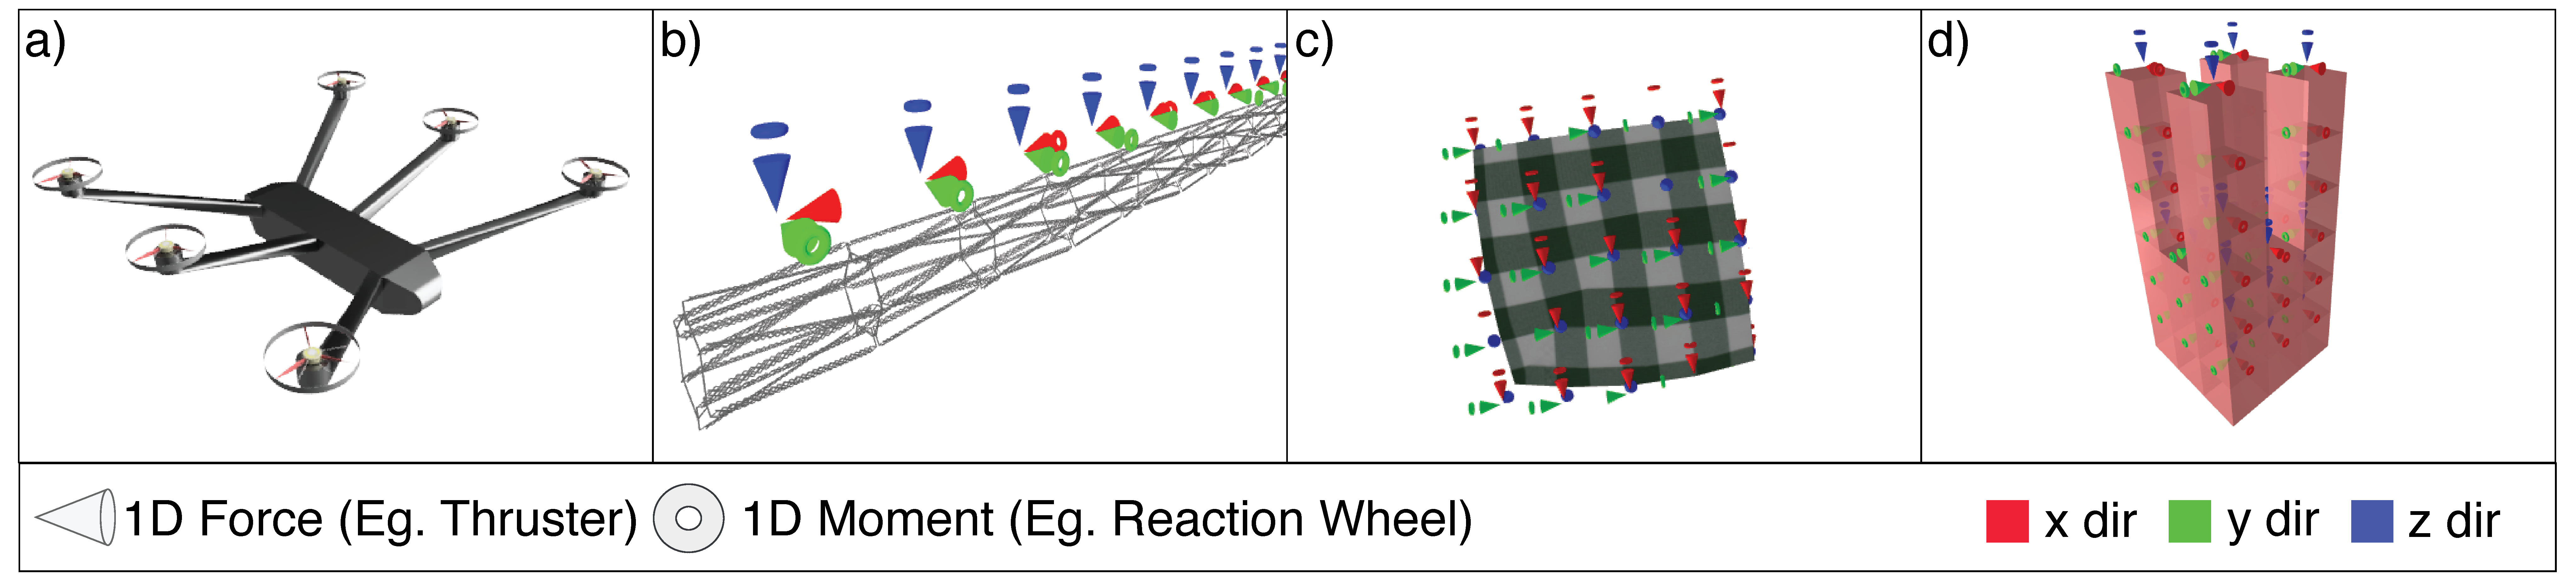
\includegraphics[width=\linewidth]{figures/Figure_5_final_solutions.eps}
    \caption{{Final actuator configurations for various optimization tasks a) the multirotor flip with a final configuration of 6 actuators placed at the extents of the body, b) 120 DoF flexible space structure with around 100 actuators placed along the body with most of the roll reaction wheels pruned, c) 150 DoF cloth manipulation with 105 force and moments applied to the various cloth nodes to achieve the desired trajectory, and d) 234 DoF soft robotic swimmer with 205 actuators along the discrete body units to enable the swimming motion. Cones represent 1-D force actuators, e.g. thruster, and toruses represent moment actuators, e.g. reaction wheel. Red represents the force/moment applied to the X-axis, Green represents the Y-axis, and Blue represents the Z-axis.}  }\label{fig:final_actuator_configuration}
\end{figure}


\begin{table}
\centering
\resizebox{\textwidth}{!}{
\begin{tabular}{|c|c|c|c|c|c|c|c|c|c|c|c|}
\hline
\begin{tabular}[c]{@{}c@{}}Low \\ Dim.\\ Tasks\end{tabular}                          & \begin{tabular}[c]{@{}c@{}}AVG\\ (STD)\end{tabular}         & \begin{tabular}[c]{@{}c@{}}CAPO\\ (ours)\end{tabular}              & GA                                                               & MIQP                                                            & MINLP                                                              & \begin{tabular}[c]{@{}c@{}}High \\ Dim.\\ Tasks\end{tabular}                                & \begin{tabular}[c]{@{}c@{}}AVG\\ (STD)\end{tabular}         & \begin{tabular}[c]{@{}c@{}}CAPO\\ (ours)\end{tabular}               & GA  & MIQP & MINLP \\ \hline
\multirow{5}{*}{\begin{tabular}[c]{@{}c@{}}Multi-\\ rotor\\ (6 DoF)\end{tabular}}    & \begin{tabular}[c]{@{}c@{}}Obj.\\ Value\end{tabular}        & \begin{tabular}[c]{@{}c@{}}1.07e8\\ (7.3e5)\end{tabular}           & \begin{tabular}[c]{@{}c@{}}1.54e8\\ (-)\end{tabular}             & -                                                               & \textbf{\begin{tabular}[c]{@{}c@{}}1.06e8\\ (2.5e5)\end{tabular}}  & \multirow{5}{*}{\begin{tabular}[c]{@{}c@{}}Space \\ Struct.\\ (120 DoF)\end{tabular}}       & \begin{tabular}[c]{@{}c@{}}Obj.\\ Value\end{tabular}        & \textbf{\begin{tabular}[c]{@{}c@{}}1.47e7\\ (31.3)\end{tabular}}    & -   & -    & -     \\ \cline{2-6} \cline{8-12} 
                                                                                     & \begin{tabular}[c]{@{}c@{}}Const.\\ Viol.\end{tabular}      & \begin{tabular}[c]{@{}c@{}}1.96e-8\\ (1.8e-8)\end{tabular}         & \begin{tabular}[c]{@{}c@{}}2.60e-9\\ (-)\end{tabular}            & -                                                               & \begin{tabular}[c]{@{}c@{}}6.37e-9\\ (9.8e-9)\end{tabular}         &                                                                                             & \begin{tabular}[c]{@{}c@{}}Const.\\ Viol.\end{tabular}      & \textbf{\begin{tabular}[c]{@{}c@{}}1.33e-14\\ (0.0)\end{tabular}}   & -   & -    & -     \\ \cline{2-6} \cline{8-12} 
                                                                                     & \begin{tabular}[c]{@{}c@{}}Runtime\\ {[}sec{]}\end{tabular} & \textbf{\begin{tabular}[c]{@{}c@{}}417.14\\ (116.27)\end{tabular}} & \begin{tabular}[c]{@{}c@{}}2996.14\\ (-)\end{tabular}            & -                                                               & \begin{tabular}[c]{@{}c@{}}1065.59\\ (514.56)\end{tabular}         &                                                                                             & \begin{tabular}[c]{@{}c@{}}Runtime\\ {[}sec{]}\end{tabular} & \textbf{\begin{tabular}[c]{@{}c@{}}423.0\\ (66.7)\end{tabular}}     & -   & -    & -     \\ \cline{2-6} \cline{8-12} 
                                                                                     & \begin{tabular}[c]{@{}c@{}}Actuator\\ Reduct.\end{tabular}  & \begin{tabular}[c]{@{}c@{}}65\%\\ (3.6\%)\end{tabular}             & \begin{tabular}[c]{@{}c@{}}12\%\\ (-)\end{tabular}               & -                                                               & \textbf{\begin{tabular}[c]{@{}c@{}}66.25\%\\ (3.4\%)\end{tabular}} &                                                                                             & \begin{tabular}[c]{@{}c@{}}Actuator\\ Reduct.\end{tabular}  & \textbf{\begin{tabular}[c]{@{}c@{}}14\%\\ (0.3\%)\end{tabular}}     & -   & -    & -     \\ \cline{2-6} \cline{8-12} 
                                                                                     & \begin{tabular}[c]{@{}c@{}}Trial\\ Success\end{tabular}     & 3/5                                                                & 1/5                                                              & 0/5                                                             & \textbf{5/5}                                                       &                                                                                             & \begin{tabular}[c]{@{}c@{}}Trial \\ Success\end{tabular}    & \textbf{5/5}                                                        & 0/5 & 0/5  & 0/5   \\ \hline
\multirow{5}{*}{\begin{tabular}[c]{@{}c@{}}Space \\ Struct.\\ (12 DoF)\end{tabular}} & \begin{tabular}[c]{@{}c@{}}Obj.\\ Value\end{tabular}        & \begin{tabular}[c]{@{}c@{}}2.710e4\\ (0.056)\end{tabular}          & \begin{tabular}[c]{@{}c@{}}2.708e4\\ (0.0\end{tabular}           & \begin{tabular}[c]{@{}c@{}}1.620e5\\ (0.0)\end{tabular}         & \textbf{\begin{tabular}[c]{@{}c@{}}2.708e4\\ (0.0)\end{tabular}}   & \multirow{5}{*}{\begin{tabular}[c]{@{}c@{}}Cloth \\ Manip.\\ (150 DoF)\end{tabular}}        & \begin{tabular}[c]{@{}c@{}}Obj.\\ Value\end{tabular}        & \textbf{\begin{tabular}[c]{@{}c@{}}9.61e5\\ (13.2)\end{tabular}}    & -   & -    & -     \\ \cline{2-6} \cline{8-12} 
                                                                                     & \begin{tabular}[c]{@{}c@{}}Const.\\ Viol.\end{tabular}      & \begin{tabular}[c]{@{}c@{}}3.11e-14\\ (0.0)\end{tabular}           & \begin{tabular}[c]{@{}c@{}}1.03e-13\\ (0.0)\end{tabular}         & \begin{tabular}[c]{@{}c@{}}0.001\\ (0.0)\end{tabular}           & \begin{tabular}[c]{@{}c@{}}8.88e-16\\ (0.0)\end{tabular}           &                                                                                             & \begin{tabular}[c]{@{}c@{}}Const.\\ Viol.\end{tabular}      & \textbf{\begin{tabular}[c]{@{}c@{}}9.7e-13\\ (0.0)\end{tabular}}    & -   & -    & -     \\ \cline{2-6} \cline{8-12} 
                                                                                     & \begin{tabular}[c]{@{}c@{}}Runtime\\ {[}sec{]}\end{tabular} & \textbf{\begin{tabular}[c]{@{}c@{}}4.059\\ (1.2)\end{tabular}}     & \begin{tabular}[c]{@{}c@{}}174.61\\ (31.23)\end{tabular}         & \begin{tabular}[c]{@{}c@{}}76.27\\ (6.55)\end{tabular}          & \begin{tabular}[c]{@{}c@{}}266.5\\ (133.10)\end{tabular}           &                                                                                             & \begin{tabular}[c]{@{}c@{}}Runtime\\ {[}sec{]}\end{tabular} & \textbf{\begin{tabular}[c]{@{}c@{}}878.0\\ (111.7)\end{tabular}}    & -   & -    & -     \\ \cline{2-6} \cline{8-12} 
                                                                                     & \begin{tabular}[c]{@{}c@{}}Actuator\\ Reduct.\end{tabular}  & \begin{tabular}[c]{@{}c@{}}10\%\\ (3.7\%)\end{tabular}             & \textbf{\begin{tabular}[c]{@{}c@{}}25\%\\ (0.0\%)\end{tabular}}  & \textbf{\begin{tabular}[c]{@{}c@{}}25\%\\ (0.0\%)\end{tabular}} & \textbf{\begin{tabular}[c]{@{}c@{}}25\%\\ (0.0\%)\end{tabular}}    &                                                                                             & \begin{tabular}[c]{@{}c@{}}Actuator\\ Reduct.\end{tabular}  & \textbf{\begin{tabular}[c]{@{}c@{}}27.5\%\\ (0.6\%)\end{tabular}}   & -   & -    & -     \\ \cline{2-6} \cline{8-12} 
                                                                                     & \begin{tabular}[c]{@{}c@{}}Trial \\ Success\end{tabular}    & 5/5                                                                & 5/5                                                              & 5/5                                                             & 5/5                                                                &                                                                                             & \begin{tabular}[c]{@{}c@{}}Trial \\ Success\end{tabular}    & \textbf{4/5}                                                        & 0/5 & 0/5  & 0/5   \\ \hline
\multirow{5}{*}{\begin{tabular}[c]{@{}c@{}}Cloth \\ Manip.\\ (24 DoF)\end{tabular}}  & \begin{tabular}[c]{@{}c@{}}Obj.\\ Value\end{tabular}        & \textbf{\begin{tabular}[c]{@{}c@{}}1.234e5\\ (0.008)\end{tabular}} & \textbf{\begin{tabular}[c]{@{}c@{}}1.234e5\\ (0.0)\end{tabular}} & \begin{tabular}[c]{@{}c@{}}1.249e5\\ (0.0)\end{tabular}         & \textbf{\begin{tabular}[c]{@{}c@{}}1.234e5\\ (0.0)\end{tabular}}   & \multirow{5}{*}{\begin{tabular}[c]{@{}c@{}}Soft \\ Robot \\ Swim.\\ (234 DoF)\end{tabular}} & \begin{tabular}[c]{@{}c@{}}Obj.\\ Value\end{tabular}        & \textbf{\begin{tabular}[c]{@{}c@{}}9.0e3\\ (46.6)\end{tabular}}     & -   & -    & -     \\ \cline{2-6} \cline{8-12} 
                                                                                     & \begin{tabular}[c]{@{}c@{}}Const.\\ Viol.\end{tabular}      & \begin{tabular}[c]{@{}c@{}}4.88e-13\\ (0.0)\end{tabular}           & \begin{tabular}[c]{@{}c@{}}2.54e-14\\ (0.0)\end{tabular}         & \begin{tabular}[c]{@{}c@{}}0.0026\\ (0.0)\end{tabular}          & \begin{tabular}[c]{@{}c@{}}1.2e-9\\ (1.6e-09)\end{tabular}         &                                                                                             & \begin{tabular}[c]{@{}c@{}}Const.\\ Viol.\end{tabular}      & \textbf{\begin{tabular}[c]{@{}c@{}}8.54e-13\\ (0.0)\end{tabular}}   & -   & -    & -     \\ \cline{2-6} \cline{8-12} 
                                                                                     & \begin{tabular}[c]{@{}c@{}}Runtime\\ {[}sec{]}\end{tabular} & \textbf{\begin{tabular}[c]{@{}c@{}}15.4\\ (2.32)\end{tabular}}     & \begin{tabular}[c]{@{}c@{}}473.1\\ (1.8)\end{tabular}            & \begin{tabular}[c]{@{}c@{}}108.12\\ (1.81)\end{tabular}         & \begin{tabular}[c]{@{}c@{}}3370.0\\ (940.0)\end{tabular}           &                                                                                             & \begin{tabular}[c]{@{}c@{}}Runtime\\ {[}sec{]}\end{tabular} & \textbf{\begin{tabular}[c]{@{}c@{}}8536.1\\ (5764.55)\end{tabular}} & -   & -    & -     \\ \cline{2-6} \cline{8-12} 
                                                                                     & \begin{tabular}[c]{@{}c@{}}Actuator\\ Reduct.\end{tabular}  & \begin{tabular}[c]{@{}c@{}}16.7\%\\ (0.0\%)\end{tabular}           & \begin{tabular}[c]{@{}c@{}}16.7\%\\ (0.0\%)\end{tabular}         & \begin{tabular}[c]{@{}c@{}}25\%\\ (0.0\%)\end{tabular}          & \textbf{\begin{tabular}[c]{@{}c@{}}37.5\%\\ (0.0\%)\end{tabular}}  &                                                                                             & \begin{tabular}[c]{@{}c@{}}Actuator\\ Reduct.\end{tabular}  & \textbf{\begin{tabular}[c]{@{}c@{}}12\%\\ (2\%)\end{tabular}}       & -   & -    & -     \\ \cline{2-6} \cline{8-12} 
                                                                                     & \begin{tabular}[c]{@{}c@{}}Trial \\ Success\end{tabular}    & 5/5                                                                & 5/5                                                              & 5/5                                                             & 5/5                                                                &                                                                                             & \begin{tabular}[c]{@{}c@{}}Trial \\ Success\end{tabular}    & \textbf{5/5}                                                        & 0/5 & 0/5  & 0/5   \\ \hline
\end{tabular}}
\caption{This table presents the results from CAPO, GA, MIQP, and MINLP on 3 low dimensional optimization tasks and 3 high dimensional optimization tasks. The table presents each method's average objective value, constraint violation, runtime, percent actuator reduction, and trial success across 5 trials. The standard deviation is presented below in parentheses. The algorithm with the best performance in a particular category are highlighted in \textbf{Bold}. CAPO was the only method that successfully solved the high-dimensional tasks.} %Results from CAPO, GA, and MIP on Benchmark Problems}
\end{table}\label{tab:benchmark_results}
% \end{minipage}

% \section{First Section}
% \subsection{A Subsection Sample}
% Please note that the first paragraph of a section or subsection is
% not indented. The first paragraph that follows a table, figure,
% equation etc. does not need an indent, either.

% Subsequent paragraphs, however, are indented.

% \subsubsection{Sample Heading (Third Level)} Only two levels of
% headings should be numbered. Lower level headings remain unnumbered;
% they are formatted as run-in headings.

% \paragraph{Sample Heading (Fourth Level)}
% The contribution should contain no more than four levels of
% headings. Table~\ref{tab1} gives a summary of all heading levels.

% \begin{table}
% \caption{Table captions should be placed above the
% tables.}\label{tab1}
% \begin{tabular}{|l|l|l|}
% \hline
% Heading level &  Example & Font size and style\\
% \hline
% Title (centered) &  {\Large\bfseries Lecture Notes} & 14 point, bold\\
% 1st-level heading &  {\large\bfseries 1 Introduction} & 12 point, bold\\
% 2nd-level heading & {\bfseries 2.1 Printing Area} & 10 point, bold\\
% 3rd-level heading & {\bfseries Run-in Heading in Bold.} Text follows & 10 point, bold\\
% 4th-level heading & {\itshape Lowest Level Heading.} Text follows & 10 point, italic\\
% \hline
% \end{tabular}
% \end{table}


% \noindent Displayed equations are centered and set on a separate
% line.
% \begin{equation}
% x + y = z
% \end{equation}
% Please try to avoid rasterized images for line-art diagrams and
% schemas. Whenever possible, use vector graphics instead (see
% Fig.~\ref{fig1}).

% \begin{figure}
% \includegraphics[width=\textwidth]{fig1.eps}
% \caption{A figure caption is always placed below the illustration.
% Please note that short captions are centered, while long ones are
% justified by the macro package automatically.} \label{fig1}
% \end{figure}

% \begin{theorem}
% This is a sample theorem. The run-in heading is set in bold, while
% the following text appears in italics. Definitions, lemmas,
% propositions, and corollaries are styled the same way.
% \end{theorem}
% %
% % the environments 'definition', 'lemma', 'proposition', 'corollary',
% % 'remark', and 'example' are defined in the LLNCS documentclass as well.
% %
% \begin{proof}
% Proofs, examples, and remarks have the initial word in italics,
% while the following text appears in normal font.
% \end{proof}
% For citations of references, we prefer the use of square brackets
% and consecutive numbers. Citations using labels or the author/year
% convention are also acceptable. The following bibliography provides
% a sample reference list with entries for journal
% articles~\cite{ref_article1}, an LNCS chapter~\cite{ref_lncs1}, a
% book~\cite{ref_book1}, proceedings without editors~\cite{ref_proc1},
% and a homepage~\cite{ref_url1}. Multiple citations are grouped
% \cite{ref_article1,ref_lncs1,ref_book1},
% \cite{ref_article1,ref_book1,ref_proc1,ref_url1}.

% \begin{credits}
% \subsubsection{\ackname} This work was supported by a NIAC award from NASA’s Space Technology Mission Directorate (Grant Number 80NSSC21K0446). Tools like ChatGPT and Grammarly were used for general editing and grammar enhancement. 

% \subsubsection{\discintname}
%  The authors have filed for a provisional patent (docket no. 2024-220) on the method described in this paper. 
% \end{credits}
%
% ---- Bibliography ----
%
% BibTeX users should specify bibliography style 'splncs04'.
% References will then be sorted and formatted in the correct style.
%
% \bibliographystyle{splncs04}
% \bibliography{CAPObib}
% %
% % \begin{thebibliography}{8}
% % \bibitem{ref_article1}
% % Author, F.: Article title. Journal \textbf{2}(5), 99--110 (2016)

% % \bibitem{ref_lncs1}
% % Author, F., Author, S.: Title of a proceedings paper. In: Editor,
% % F., Editor, S. (eds.) CONFERENCE 2016, LNCS, vol. 9999, pp. 1--13.
% % Springer, Heidelberg (2016). \doi{10.10007/1234567890}

% % \bibitem{ref_book1}
% % Author, F., Author, S., Author, T.: Book title. 2nd edn. Publisher,
% % Location (1999)

% % \bibitem{ref_proc1}
% % Author, A.-B.: Contribution title. In: 9th International Proceedings
% % on Proceedings, pp. 1--2. Publisher, Location (2010)

% % \bibitem{ref_url1}
% % LNCS Homepage, \url{http://www.springer.com/lncs}, last accessed 2023/10/25
% % \end{thebibliography}
% % \end{document}


%%% Local Variables:
%%% coding: utf-8
%%% mode: latex
%%% TeX-engine: xetex
%%% TeX-master: "../thesis"
%%% End: